\documentclass[12pt]{article}
\linespread{1.5}
\pdfminorversion=6

\usepackage{booktabs}
\usepackage{tabularx}
\usepackage{caption}
\usepackage[flushleft]{threeparttable}
\usepackage{threeparttablex}

\usepackage[english]{babel}
\usepackage{float,color}
\usepackage[pdftex]{graphicx}
\usepackage{hyperref}
\usepackage{graphicx,scalerel}
\hypersetup{colorlinks,linkcolor=black,urlcolor=blue,citecolor=black}
\usepackage{amssymb}
\usepackage{amsmath}
\usepackage{placeins}
\usepackage[format=hang,font=normalsize,labelfont=bf]{caption}
\usepackage[margin=1in]{geometry}
\usepackage{url}
\usepackage{listings}
\usepackage{amsxtra}
\usepackage{setspace}
\usepackage{authblk}
\usepackage{csquotes}

% Bibliography stuff
\usepackage[
hyperref=true,
giveninits=true, % render first and middle names as initials
uniquename=init,
maxcitenames=3,
maxbibnames=99,
style=authoryear,
dashed=false, % re-print recurring author names in bibliography
natbib=true,
useprefix=true, % for inclusion of 'de' 'da' in surname
urldate=long,
backend=biber,
style=apa]{biblatex}
\addbibresource{bibliography.bib}


% adds space above row
\newcommand{\customlinespace}{\addlinespace[.1cm]}

% command for all table/figure notes
\newcommand{\Fignote}[1]{
	\begin{tablenotes}[para,flushleft]\footnotesize
		\textit{Note}: #1
	\end{tablenotes}
}

% stars
\newcommand{\sym}[1]{\rlap{#1}}

% note addendem for fixed effects
\newcommand{\FEnote}{All specifications include household and month fixed effects. }

% note addendem for regression tables
\newcommand{\Regnote}{Standard errors in parentheses are clustered at the zip code level. ***, **, and * indicate significance at the 1, 5, and 10 percent critical levels, respectively.}


% Title page stuff
\title{The Effect of the Cook County, Illinois Tax on Sugar-Sweetened Beverages on Sugar Consumption}
\author{Zachary A. Goodman\thanks{zgoodman@ucsd.edu}\\ and Jacob Orchard\thanks{jdorchard@ucsd.edu. We gratefully recognize Prashant Bharadwaj, Jeffrey Clemens, Gordon Dahl, Itzik Fadlon, Mark Jacobsen, Katherine Meckel, Kaspar Wuthrich, and numerous seminar participants for their helpful comments and suggestions. We thank Eric Youn for outstanding research assistance. Our analyses are calculated based in part on data from Nielsen Consumer LLC and marketing databases provided through the NielsenIQ Datasets at the Kilts Center for Marketing Data Center at The University of Chicago Booth School of Business. The conclusions drawn from the NielsenIQ data are those of our own and do not reflect the views of NielsenIQ. NielsenIQ is not responsible for, had no role in, and was not involved in analyzing and preparing the results reported herein.}}
\affil{University of California, San Diego}
\date{This version: May 2021\\
First Version: June 2019}

\begin{document}
\maketitle

\begin{abstract}

Do taxes on sweetened beverages decrease sugar consumption? We examine the effects of the largest experiment in sweetened beverage taxes (in Cook County, Illinois) and the only one revoked as of this writing. We combine household scanner data with barcode-level nutrition data, which allows us to observe household nutrient bundles during the tax in addition to purchases of taxed beverages. We find that while the tax is active, consumers decreased their sugar purchases from all sources by 14.9\%, most of which is explained by decreases in sugar from regular soda and fruit drinks. We document significantly larger decreases in sugar purchases for households who live far from the Cook County border and households with high pretax levels of regular soda purchases. In the months following removal of the tax, we find that households returned to pretax-levels of sugar consumption, suggesting that four months is not long enough to expect sustained behavioral change in this context. Finally, we develop a simple household model to weigh the welfare consequences of the tax's potentially positive health effects with the associated increase in consumer prices. We find that the tax increased the cost of living by approximately 2 cents per gram of sugar reduction.
\end{abstract}

\pagebreak

%%%%%%%%%%%%%%%%%%%%%%%%%%%%%%%
% Introduction
%%%%%%%%%%%%%%%%%%%%%%%%%%%%%%%
\doublespacing

\section{Introduction} \label{introduction}

Obesity remains among the costliest health issues in the United States today. \textcite{finkelstein2009annual} find that obesity-related health expenses cost the U.S. between \$107 billion to \$184 billion in 2008 in 2018 dollars. \textcite{cawley2012medical} estimate significantly larger aggregate expenses totaling \$261 billion using an IV approach. As a potential solution to reducing the high medical costs of obesity, government agencies have relatively recently suggested reducing added sugar consumption \parencite{dietary2015dietary}. Sugar sweetened beverages (SSBs) are the source of nearly 40\% of the average American's consumption of added sugar \parencite{dietary2015dietary} and about 7\% of caloric intake \parencite{allcott2019should}. Several policymakers have recommended imposing taxes on sweetened beverages to reduce sugar consumption and associated health costs, a strategy that has worked for other harmful-to-health products like tobacco \parencite{chaloupka2012tobacco}.

While excise taxes on soft drink taxes have existed for many years in the U.S. and other countries, beverage taxes levied at the \textit{ounce} level have been passed in eight U.S. localities starting with Berekely, California in 2015.\footnote{For expositional ease, \textit{beverage tax} hereafter refers to the class of beverage taxes levied at the ounce level.} In this paper we focus on the largest of these localities, Cook County, Illinois, which enacted and revoked a one-cent-per-ounce tax on sweetened beverages in 2017. As the only sweetened beverage tax revoked in the United States as of this writing, Cook County's tax is uniquely interesting for studying the effects of short-term taxes on long-term behavioral change. Additionally, Cook County's tax affected the largest population among all beverage taxes in the U.S., allowing for increased precision of effect estimators.

While other researchers have estimated the effects of beverage taxes on beverage demand and sugar from beverages, few have examined the impact on the policy-relevant metric of total sugar consumption. It is important to consider the complete basket of foods consumed when estimating the effects of taxes on nutrients: examining only the taxed product class in isolation may overstate the effects of the tax if consumers substitute towards other food product classes (for example if consumers substitute from taxed soda to untaxed cookies). On the other hand, if the tax carries a signal that causes consumers to update their priors about the healthfulness of a particular product attribute, then the estimated effects could be \textit{understated}.

Unfortunately, it is challenging to reliably observe nutrient consumption across all foods over an extended period of time. Common methods, such as surveys and food diaries, suffer from small sample sizes, limited time frames, and high measurement error from poor recall and incorrect labeling. To overcome this limitation, we use a large representative panel dataset with barcode-level information about the products \textit{purchased} in a household. We then match these data with barcode-level nutrition panel data to observe nutrients purchased over time within a household. While nutrient consumption and nutrient purchases are not equivalent, we treat purchases as a proxy for consumption.

Our primary outcome measure of interest is grams of sugar purchased, both during the tax and shortly after the tax is removed. We exploit variation across time and geography in a differences-in-differences specification to conduct our analysis. Specifically, we use households residing in the Chicago Designated Market Area (DMA)\footnote{Nielsen's DMAs are similar to the Census Bureau's Metropolitan Statistical Areas.} as our primary counterfactual for households living inside Cook County. We construct a second counterfactual composed of the top ten largest counties by population (other than Cook County). While the first counterfactual shares region-specific shocks with Cook County, the second counterfactual is less likely to suffer from spillover effects and other violations of the Stable Unit Treament Value Assumption (SUTVA).

We find that on average, the Cook County beverage tax reduced sugar purchases from all foods by 14.9\% compared to those households outside the border. The results are similar when using large counties as the counterfactual, albeit somewhat smaller magnitudes. We find no evidence that the tax caused reductions in sugar purchases that persisted after the tax was removed, nor do we find an increase beyond pretax levels of sugar. Similar to other authors, we find that the taxes decreased purchases of taxed beverages across both extensive and intensive margins. However, unlike prior work, we confirm that the reduction in sugar purchases is explained almost entirely by taxed products, suggesting that substitution towards untaxed products is likely modest for most households.

We examine heterogeneity across several dimensions. First, we find that reductions in sugar are largest for the poorest households in our sample, and we find no differences in reductions across race or education dimensions. Second, we estimate the effects of the tax as a function of distance from a household's zip code to the Cook County border, and we find smaller and statistically insignificant effects for households on the border and larger and significant effects for households residing further inside the border. Finally, we estimate the effects of the tax as a function of pretax levels of soda purchases. While the tax had no statistically significant effect on sugar purchases for low-soda households, the tax had large and significant effects on the top three deciles of households by pretax soda purchases.

Finally, we compare the SSB taxes possible benefits of reduced sugar consumption with its main cost: an increase in consumer prices. Specifically, we develop a simple household model where the household has CES preferences over a range of products, some of which are taxed. We estimate the households implicit price index before and after the tax in Cook County and our counterfactual (Chicago DMA sans Cook County) and find that the tax cost the representative household between \$7.63 and \$24.21 during the four month period of the tax. While the tax decreased sugar consumption by a significant amount, the reduction came at the cost of approximately 2.1 to 6.6 cents per gram.
% Although most of the SSB taxes passed in the U.S. were passed by voter referenda, the policies have been highly controversial. Proponents of these measures have argued that like taxes on tobacco products, taxes on SSBs could be effective in improving public health. Opponents have argued that these taxes are poorly targeted, allowing for evasion through cross-border shopping and consumption of sugar through other products beyond beverages. Additionally, opponents have contended that the taxes may be regressive as beverages constitute a larger share of poorer consumers' budgets than they do for those with more resources.

The remainder of the paper is organized as follows. Section \ref{background} provides a background of the policies enacted and related literature. Sections \ref{methods} and \ref{data} introduce the methods and data used, respectively. Section \ref{results} summarizes our results. Section \ref{discussion} concludes with a discussion of those results.

%%%%%%%%%%%%%%%%%%%%%%%%%%%%%%%
% Background
%%%%%%%%%%%%%%%%%%%%%%%%%%%%%%%
\section{Background and Related Literature} \label{background}

In this section, we provide background on beverage taxes and summarize existing related literature.

\subsection{Beverage taxes in the United States}

While dozens of cities have considered taxing beverages, the first city to enact a beverage tax was Berkeley, California in March 2015. Berkeley's Measure D levied a one-cent-per-ounce excise tax on the distribution of beverages with added sugar. Alcohol, milk products, beverages for medical use, 100\% fruit and vegetable juices, water, and artificially sweetened beverages are all exempt from the tax. Nearly two years after Berkeley, other cities began enacting similar SSB taxes including Philadelphia, PA, (2017); Oakland, CA, (2017); Albany, CA (2017); Boulder, CO, (2017); San Francisco, CA, (2018); Seattle, WA, (2018). Cook County became the first county to enact a county-wide beverage tax on August 2, 2017. Two months later on December 1, the county became the first locality in the United States to remove an SSB tax. One can observe a timeline of SSB tax events in Figure \ref{taxtimeline}.

\begin{figure}[t]\centering
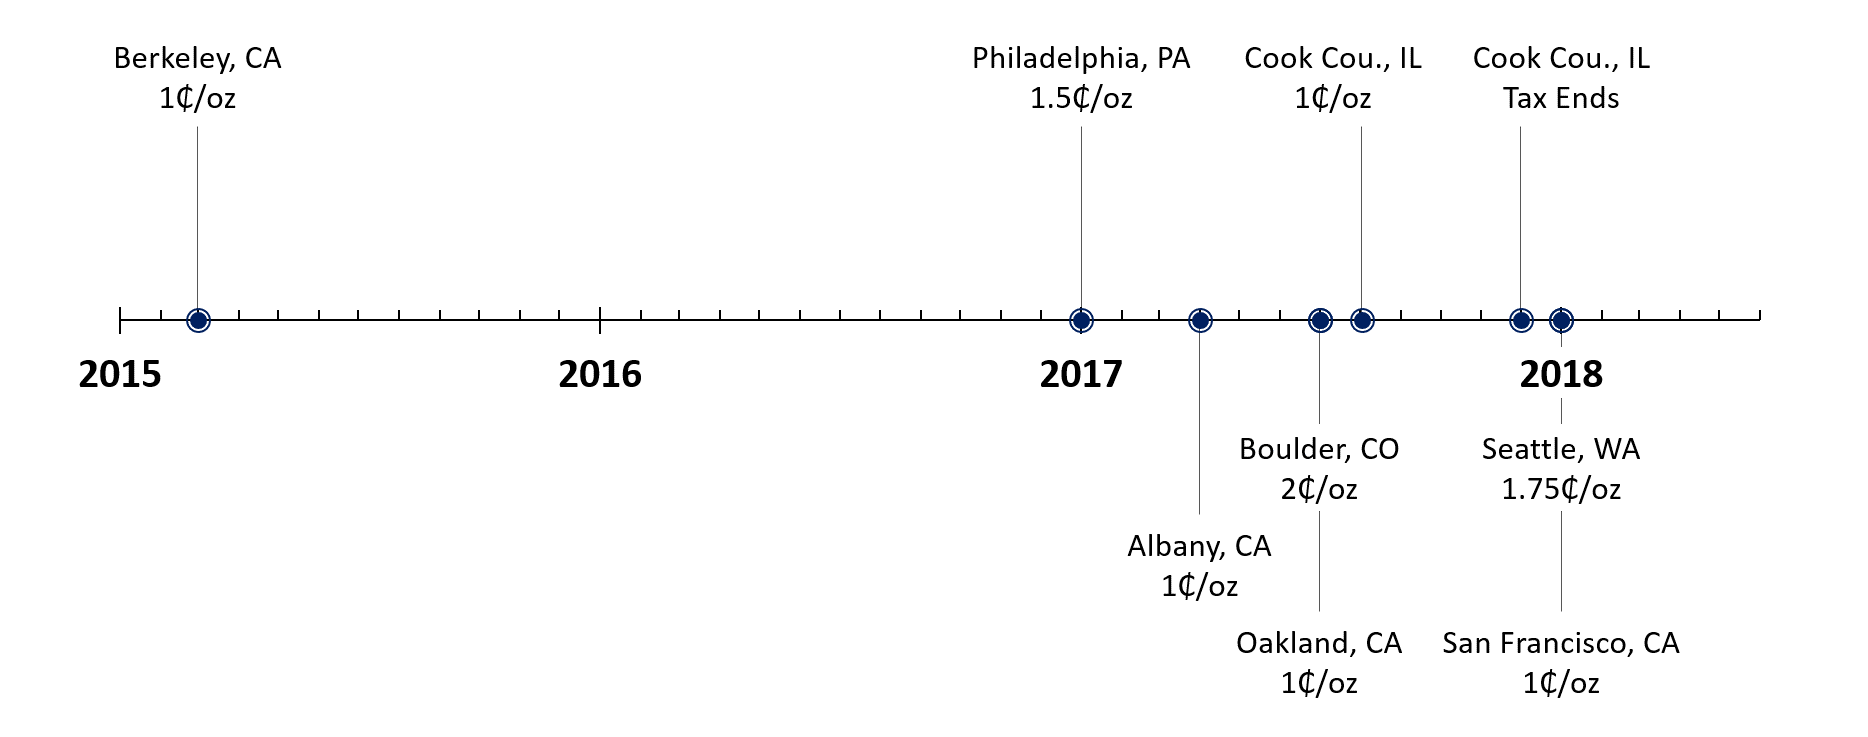
\includegraphics[width = \textwidth]{../figures/taxtimeline.png}
\caption{Rollout of beverage taxes in the United States \label{taxtimeline}}
\end{figure}

The Berkeley tax is the longest standing SSB tax in the U.S. and the most studied for its impact on consumption. \textcite{falbe2015higher} randomly surveyed retail establishments in San Francisco, Oakland, and Berkeley both before and after the tax change and found that the one-cent-per-ounce tax led to 0.46-0.67 cent increase in the price per ounce, depending on the type of beverage. In a follow-up study, \textcite{falbe2016impact} used a repeated cross-sectional survey of low-income and minority households before and after the tax. Participants were asked how often they consume different types of beverages each week or month, and total SSB consumption was inferred from their responses. The authors found that SSB consumption decreased by 21\% in Berkeley while it increased by 4\% in comparison cities. \textcite{silver2017changes} used store surveys and point-of-sale scanner data for three Berkeley and six non-Berkeley supermarkets to assess the tax pass through. They found that the tax pass-through was near 100\% for large chain supermarkets and smaller for others. They also found that sales of SSBs decreased in Berkeley relative to other cities. \textcite{cawley2017berkeley} add to the literature that stores in Berkeley pass through more of the tax to consumers the further away they are from borders with neighboring untaxed localities, ceteris paribus.

Each of the aforementioned studies find evidence that the tax in Berkeley resulted in high, but not 100\%, pass-through of the tax to consumers, which reduced SSB consumption. From these findings we learn that consumers are not perfectly elastic in their demand for SSBs, but we cannot say whether the taxes reduced sugar consumption because the authors did not examine demand interrelationships with other goods that contain sugar. While about 39\% of the average American's daily sugar consumption \parencite{dietary2015dietary} and about 7\% of daily calories \parencite{allcott2019should} come from beverages that are taxable under the examined policies, it would be a problem for policymakers if, for example, taxed consumers substituted away from soda towards chocolate milk or candy. Most of these studies also suffer from only sampling consumers in one region and failing to track where consumers purchase SSBs, which may have changed following the tax. Additionally, these studies rely on survey data, which likely contain significant response bias. Given the increased attention of the potential negative health effects of SSBs and respondents' tendencies to provide prosocial answers to surveyors\footnote{Researchers have observed that people tend to overreport socially positive behaviors like voting \parencite{silver1986overreports} and attending church \parencite{hadaway1993polls} but underreport socially negative behaviors like declaring bankruptcy \parencite{locander1976investigation} and using illegal drugs \parencite{mensch1988underreporting}. See \textcite{krumpal2013determinants} for a review of the literature on ``Social Desirability Bias."}, it would not be surprising to find that respondents underreport their SSB consumption to a larger degree following implementation of the tax.

More recently, other authors have examined the SSB taxes in Boulder \parencite{cawley2021boulder}, Oakland \parencite{cawley2020oakland}, and Philadelphia \parencite{cawley2020philly}. In Boulder, Cawley and coauthors find that nearly 80\% of the two-cents-per-ounce tax in Boulder was passed on to the consumer. Importantly, they note that about one-fifth of the retailers surveyed added the SSB tax at the register rather than into the shelf-price, which may have reduced saliency of the tax, perhaps lowering its effectiveness \parencite{chetty2009salience}. In Oakland, the authors find that the one-cent-per-ounce tax was passed through at a rate of about 60\% and did not statistically significantly decrease sweetened beverages purchased per trip or added sugar consumed from beverages. In Philadelphia, the authors find that consumers purchased 8.9 ounces of SSBs per shopping trip less from stores within the city relative to consumers who purchased SSBs from stores outside the city. They also find evidence that city residents increased their purchases of SSBs outside the city. \textcite{cawley2020impact} estimate the effects of SSB taxes in four cities (Oakland, Philadelphia, San Francisco, and Seattle) on consumer purchases using household receipt data from InfoScout. They find that a one-cent-per-ounce increase in tax rate reduces purchases of taxed products by 12.2\%, driven primarily by panelists in Philadelphia.

\subsection{Cook County's beverage tax}

Here we review the history of the Cook County beverage tax and provide specific details about timing and implementation.

The Cook County Board of Commissioners passed the Cook County Sweetened Beverage Tax Ordinance with a 9-8 vote on November 10, 2016. Initially, the one-cent-per-ounce tax was slated to go into effect on July 1, 2017; however, four days earlier on June 27, the Illinois Retail Merchants Association filed suit, questioning the constitutionality of the tax. A state judge issued a temporary restraining order on the new tax until the case could be reviewed. On July 28, the same judge dismissed the lawsuit, and shortly thereafter on August 2, 2017, the beverage tax went into effect. As Cook County is home to 5.2 million residents, this tax became the most widespread beverage tax in the United States.

The Cook County beverage tax is unique among the other beverage taxes in the U.S. Besides having impacted the largest U.S. population to date, the law required that the tax be ``borne by the purchaser of the sweetened beverage," \parencite{cookcounty2016}. In practice, this meant that although the tax was collected by distributors, the law required that the tax be added to the price faced by consumers, usually in the form of a line-item on the receipt. This element of the policy has important implications for pass through and salience. Several large chain retailers added to the price tags of beverages a disclaimer that the tax would be added at the register (see Appendix \ref{pricetag} for an example.) However, it is possible that many retailers added the tax at checkout without including the tax in the displayed price, which may have reduced salience of the tax and possibly the impact on consumption \parencite{chetty2009salience}.

Another difference between the Cook County tax and beverage taxes in other localities is the taxation of both regular and diet beverages. Besides Philadelphia, Pennsylvania, Cook County is the only other locality in the US to have included diet beverages in its beverage tax. Since diet beverages are close substitutes for regular beverages but contain no sugar, taxing them may be counterproductive if the goal is reduced sugar consumption. On the other hand, if increasing tax revenue is part of the objective function, then taxing diet beverages may be a dominant policy strategy.

To grasp the magnitude of the tax in Cook County, consider some popular beverages from our data. The most popular (in gross sales) carbonated beverage in our data for Cook County consumers is a 12-pack of 12-ounce cans that retails for \$3.57 on average. The Cook County beverage tax adds \$1.44, or 40\%, to the price of this 12-pack on average. The most popular two-liter carbonated beverage retails for \$1.42 on average, and the tax adds 48\% to the price of this 67.6-ounce product. Across all carbonated beverages purchased in our dataset, we estimate the average percent tax to be about 23.5\%.\footnote{We only include carbonated beverages in this calculation since nearly all carbonated beverages are taxed whereas other beverage categories include both taxed and untaxed products (e.g. 100\% fruit juices are exempt but share a category with fruit-flavored drinks).}

It is worth noting that Chicago levies a 3\% tax on non-fountain soft drinks (added at the register) as well as a 9\% tax on wholesale fountain drink syrups (paid by distributor) since 1994. Beverages in Chicago are also subject to an Illinois state sales tax of 6.25\%, Cook County sales tax of 1.75\%, Chicago sales tax of 1.25\%, and a Regional Transit Authority tax of 1\%. The beverage tax studied in this paper is in addition to these aforementioned taxes, which remain constant during the period of study.

Importantly, sweetened beverages purchased using SNAP benefits were exempt from the Cook County beverage tax since federal law prohibits taxation of products purchased using SNAP. All other localities in the US that have enacted beverage taxes levied them on distributors and did not require that the tax be added at the register. Hence, the passed-through portion of the taxes in these localities could be paid for using SNAP benefits. Given this difference, it is plausible that effects of the beverage tax in Cook County could have been smaller for the poorest households relative to effects of similar taxes in other localities. Another element to consider is that poor households most likely to receive SNAP benefits are also those most likely to face the nutrition informational barriers that drive internalities from SSB consumption \parencite{allcott2019should}. If so, then exempting SNAP benefits from the tax may actually hurt the poorest consumers.

On October 11, 2017, the Cook County Board of Commissioners voted 15-2 to repeal the ordinance, becoming the first governing body in U.S. history to revoke a beverage tax. The one-cent-per-ounce tax expired on December 1, 2017.

\subsection{Theoretical rational for beverage taxes}

Medical researchers have presented evidence that excess sugar consumption is strongly associated with metabolic-related diseases such as obesity and type 2 diabetes, dental carries, and cognitive decline \parencite{malik2010sugar, imamura2015consumption, malik2019sugar}. Additionally, several randomized trials have demonstrated a causal link between reduced SSB consumption and improved health \parencite{ebbeling2006effects, vartanian2007effects, ebbeling2012randomized, de2012trial}. \textcite{wang2012penny} and \textcite{long2015cost} both estimate that each ounce of SSB consumed carries with it approximately one cent of health system cost. If the health system collects these costs from consumers of health care, then there would not be externalities from harmful effects of SSBs on health. On the other hand, if these costs are not covered by consumers themselves, then taxes on beverages could help pass the social costs of SSB consumption to the consumer.

\textcite{cawley2012medical} find that about 88\% of obesity-related medical expenses are paid for by parties other than the consumer of the health care. Taking this estimate along with those of \textcite{wang2012penny} and \textcite{long2015cost}, \textcite{allcott2019regressive} estimate that the external cost of SSB consumption is in the range of 0.8 to 0.9 cents per ounce.

If one takes the perspective of a social planner seeking to maximize long-term welfare, as \textcite{allcott2019regressive}, then consumers may face \textit{internalities} from their own myopia and overconsumption of SSBs, which carry costs in the hyperbolically-discounted future. Additionally, information frictions may impose internalities; that is, consumers might consume fewer SSBs if they have the same knowledge of the health effects as do dietitians and nutritionists. Allcott and coauthors estimate that, in dollar terms, the marginal internality from SSB consumption is 0.9 to 2.1 cents per ounce. In sum, the authors suggest that the optimal federal beverage tax is between 1 and 2.1 cents per ounce, or around 0.4 cents per ounce if only considering externalities. Note that this ``optimal tax'' is reduced from the sum of the externalities and internalities by taking into account the regressive financial cost of the tax, which reduces the optimal tax by about 0.5 cents per ounce. For city-level taxes, the authors suggest that the optimal tax may range 0.5 to 1 cent per ounce to account for 50\% and 25\% cross-border shopping, respectively.

%%%%%%%%%%%%%%%%%%%%%%%%%%%%%%%
% Data
%%%%%%%%%%%%%%%%%%%%%%%%%%%%%%%
\section{Data} \label{data}

We identify the effects of SSB taxes by linking several data sources. First, we observe household-level food purchase and demographic data from the Nielsen Homescan Survey, a nationally representative panel of 40-60,000 households from 2004 to 2016. These data have been used to asses the effects of other taxes. \textcite{harding2012heterogeneous} use the homescan data to asses the impact of cigarette taxes, especially for panelists living close to state borders. \textcite{cotti2016effects} look at how tobacco taxes affect smoking cessation product purchases. \textcite{dharmasena2012intended} assess the effects of a hypothetical tax on sugar. \textcite{colchero2016beverage} and \textcite{colchero2017mexico} use Nielsen panel data in Mexico to evaluate the impact of a one-peso per liter tax on SSBs.

Nielsen provides recruited households with a handheld barcode scanner and asks them to record every item they purchase. By scanning their purchased products, households earn points that can be redeemed in a rewards catalog much like credit card reward programs. The households can earn higher value rewards the longer they remain in the panel, so households are additionally incentivized to participate in the panel for multiple years (the median household participation duration is about 7 years). Nielsen collects household characteristics including zip code level geographic identifiers, household size, age of household members, race, income range, and more. In Table \ref{summary_table}, we present descriptive statistics of households in the Chicago DMA sample by treatment status.

Participants are asked to scan the UPC codes of \textit{all} the products they buy following shopping trips and provide information on the location of the purchase. If the purchase was completed at a Nielsen partner retail outlet, the price of the purchased item is automatically recorded as the average price of that product during the week that the customer recorded the purchase. If the purchase was made at a non-participating retail outlet, the participant is asked to manually input the price. If the product does not have a barcode as is the case with raw fruits and vegetables, households can record their purchase by scanning a barcode for the corresponding item printed in a provided booklet. Given that households may forget or choose to omit recording some of their purchases, the Nielsen Homescan Survey data likely contain measurement error. However, provided the measurement error is uncorrelated with introduction of SSB taxes, our findings, presented as percent changes, should remain unbiased. Levels of consumption presented in the data should be considered underestimates given the high likelihood of under-reporting by households \parencite{einav2010recording}.

We match the UPC codes from purchases in the Nielsen data with product-level nutrition data, thereby permitting us to observe total quantities of nutrients purchased by each household per month. Our nutrition data come from three sources. First, we use proprietary nutrition data from Syndigo, who provide UPC-level product information including the Nutrition Facts (amount of each micro and macronutrient listed), ingredients, product size, description, and brand for over 220,000 branded packages.\footnote{The data are licensed by over 2,000 consumer applications and have been used to estimate nutrients purchased by Nielsen panelists by other authors including \textcite{dubois2014prices}.} We use an imputation procedure, described next, to match similar products that do not have a direct UPC match. Second, we use the US Department of Agriculture's FoodData Central to gather nutrition information for as many of the remaining products as possible. Finally, for all remaining products, we use the search features of major online retailers to find images of the Nutrition Facts panel and manually record the information.

To match nutrition data to the Nielsen product data, we follow a procedure similar to that of \textcite{dubois2014prices}. We first drop non-food products, alcohol, tobacco, weight-loss/diet aids, and reference card goods.\footnote{Reference card goods are products without a barcode that panelists can report they purchased by scanning barcodes listed in a barcode reference booklet. These reference barcodes are associated with pictures and standardized item descriptions (such as ``bakery item"). We drop these products since we cannot infer accurate nutrition information, and reference card goods are vastly underreported relative to products that have barcodes. Nielsen provides alternative panelist weights for analyses that include reference card goods.} We then merge on UPC code, which matches about 52.8\% of the purchased UPCs. Next, for products without a direct match, we match within product (string description of the product), brand, product module,\footnote{over 1,000 product categories defined by Nielsen}, size type (measured in counts versus milliliters versus grams), flavor, variety, type, formula, and style. This step adds 23.8\% to the matched data. Next, we relax the brand requirement, which permits matching of store-brand goods and adds 11.2\% of purchased products.\footnote{The Syndigo data do not include store-brand goods.} Next we relax the flavor, variety, type, formula, and style requirements, which allow for another 7.6\% of products to be matched. For 4.0\% of products, we impute within product module for those product modules that have sufficient matched observations. For the remaining product modules, or 0.5\% of purchased products mostly comprised of fresh produce, we manually look up and enter nutrition information.

To reduce the influence of outliers, we topcode our aggregated nutrient measures at the 99th percentile for all values greater than the 99th percentile.

%%%%%%%%%%%%%%%%%%%%%%%%%%%%%%%
% Methods
%%%%%%%%%%%%%%%%%%%%%%%%%%%%%%%

\section{Methods} \label{methods}

In this section, we describe the empirical strategies used in this paper.

\subsection{Effect on food and nutrient purchases}

We use a differences-in-differences specification to examine the impact of the beverage tax on food and nutrient purchases. We compare the change in monthly purchases during the taxed period by households living in Cook County, Illinois to that among counterfactual households. Our specification is as follows:

\begin{align}
	y_{it} = \beta_1 \tau_{s(i)t} + \gamma_i + \delta_t + \epsilon_{it} \label{spec_did}
\end{align}

where $y_{it}$ is the total purchases of a food or nutrient $y$ by household $i$ during month $t$, $\gamma_i$ and $\delta_t$ are household and time fixed effects, respectively, and $\epsilon_{it}$ is an unobserved model residual. $\tau_{s(i)t}$ is the beverage tax in a locality-month with units cents-per-ounce where $s(i)$ is the locality where household $i$ resides. Under the parallel trends assumption, unconfoundedness, and SUTVA, the coefficient of interest, $\beta_1$, is interpreted as the average causal effect of the tax on monthly purchases of $y$ during the observed taxed period. In practice, we will take the inverse hyperbolic sine of $y$ such that our results can be interpreted as percent changes.

Choosing a counterfactual that satisfies all of the assumptions aforementioned is challenging. In our preferred specification, we use Chicago DMA households that reside outside of the Cook County border as the counterfactual. While it is reasonable that households in the same DMA likely experience similar region-specific shocks thereby increasing the plasubility of the parallel trends and unconfoundedness assumptions, SUTVA is potentially less reliable. For example, it is conceivable that control households may shop at grocery stores inside Cook County, or stores outside the border offer promotions or increase marketing to attract additional business during the taxed period. Hence, we additionally estimate our specifications using households who reside in the top ten largest U.S. counties by population, other than Cook County and other counties that pass or enact a beverage tax during the period studied. While it is less plausible that households in distant counties experience similar regional shocks, it is reasonable to expect that these households are insulated from spillovers from the Cook County beverage tax.

To examine heterogeneous treatment effects, we add an interaction term to Equation \ref{spec_did}:

\begin{align}
	y_{it} = \beta_1 \tau_{s(i)t} + \beta_2 \text{I}_{i} \tau_{s(i)t} + \gamma_i + \delta_t + \epsilon_{it} \label{spec_het}
\end{align}

where $\text{I}_{i}$ is a household-specific, time-invariant covariate of interest. Specifically, we add interaction terms with key demographic variables, such as household income, to identify if the tax may have had differential effects across these demographic variables. Household income is of particular interest, besides for examining the potential regressivity of the tax, since beverages purchased with SNAP benefits were exempted from the tax.\footnote{We cannot directly observe whether SNAP benefits were used to pay for products, but we can observe household income ranges as well as if an alternative to cash and credit was used. Unfortunately, fewer than 100 households in our treatment sample can be classified as SNAP-eligible households, and an even smaller subset of these use cash and credit alternatives. Hence, we focus our analysis examining heterogeneity along income ranges.}

We also estimate Equation \ref{spec_het} with $\text{I}_{i}$ as percentiles of pretax levels of regular soda purchases, scaled by the inverse of total monthly expenditures. In this specification, $\beta_2$ identifies the difference in treatment effects for high soda purchasing households to those that do not purchase soda. Low soda-purchasing households in Cook County can be thought of as an additional control group since they face less exposure to the tax yet experience the same county-specific shocks that high soda-consuming households experience.\footnote{Regular soda was not the only beverage taxed, so these households may have still experienced some exposure to the tax.}

Finally, given the potential for Cook County residents to purchase beverages across the border, we estimate Equation \ref{spec_het} setting $\text{I}_{i}$ as indicators for the household's ``layer" within the county, thereby helping us understand whether the tax had larger effects for those further from the border. We code all households in our sample using their residential zip code to be one of five categories: outside border, cross border, on border, and two inside-border categories depending on linear distance to the nearest untaxed zip code. We depict these layers in Figure \ref{cookzip}. In our analysis, we drop the 50 cross-border households given their small numbers and unclear taxed status.\footnote{Including an indicator variable for this group in our specifications has little influence on the results, and we do not have ample precision to draw any conclusions from this group.} We omit an indicator for outside-border households, and hence all coefficients are interpreted as the average change in purchases during the tax for a given layer relative to outside-border households.

When estimating Equations \ref{spec_did} and \ref{spec_het}, we cluster our standard errors at the zip code level to allow for arbitrary serial correlation of residuals among households in the same zip code over time. While the Cook County beverage tax was levied at the county level, we are unable to reliably cluster our errors at such fine a level since our sample is comprised of too few counties. Additionally, we weight households in our sample using a Nielsen-provided projection factor, which helps make the panel more representative of the general U.S. population.\footnote{Uniformly weighting each household has a small but not substantive impact on the results.} Finally, for months where a household has zero store trips and purchases, we code observations as missing. To check that our results are not substantially biased by potentially nonrandom missing purchase data, we estimate our specifications restricted to a subsample of panelists that have at least one purchase per month.

\subsection{Welfare}

While the above methods help us understand whether the tax may reduce sugar consumption and improve health, they do not capture the implicit costs to households in terms of an increase in their price index. In order to examine the welfare costs of the tax, we develop a simple household model where households derive utility from grocery consumption and from their health. Some of the health effects of sugar are non-internalized, which induces the policy maker to impose a tax. The household's utility is given as:

\begin{align}
	U(C_t,H(S_t)) = \log(C_t) + \alpha H(S_t)
\end{align}
where H$(\cdot)$ is a function of sugar on the health of the consumer that is not internalized. C is a nested CES aggregation of $N_m$ grocery goods within M different categories:

\begin{align}
	C_t = \left( \sum_m^M \left( \sum_k^N (\varphi_{k,t} c_{k,t})^{\frac{\sigma_m-1}{\sigma_m}}\right)^{\frac{\sigma_m}{\sigma_m-1}} \right)^{\frac{\sigma}{\sigma-1}}.
\end{align}

The household derives utility from consumption of each product at time t $c_{k,t}$. This per product utility varies with time specific taste shocks for each product $\varphi_{k,t}$. This taste parameter is meant to represent all of the internalized utility that the household derives from the product (including its health benefits). So if the sugar tax increases the household's knowledge about the negative health effects of sugar than we might expect $\varphi$ to decrease for products with high amounts of sugar. Each product group has it's own specific elasticity of substitution $\sigma_m$ and there is another elasticity of substitution across product categories $\sigma$.

Following standard CES optimization, each product category m has price index at time t of:

\begin{align}
P_{tm} = \left[ \sum_k \left( \frac{p_{k,t}}{\varphi_{k,t}}\right)^{1-\sigma_m}\right]^{\frac{1}{1-\sigma_m}}. \label{priceindex_simple}
\end{align}

What matters for the household's price index is the taste adjusted price of the good $\frac{p_k}{\varphi_k}$ rather than simply the price. This is important for our analysis as the tax increases the price of SSB, but can also affect the ``taste'' for sugar given that the tax may signal to consumers that sugar is a bad. It should be noted that both the taxes affect on increasing the price of SSB as well as decreasing the taste for sugar will both act to increase the consumer's price index. So the price index could increase even more than the simple case depending on the consumer's ability to substitute to other goods.

We use the reverse weighting method from \textcite{redding2020measuring} to calculate the elasticity of substitution for each product module $\sigma_m$ and the elasticity of substitution across product modules $\sigma$ using all of the data in our sample (both inside and outside Cook County). We also follow \textcite{redding2020measuring} and invert the price index in \eqref{priceindex_simple} so that we do not need to estimate the time specific good taste parameter $\varphi_{k,t}$. The change in the price index in a product category m between any two periods then becomes:

\begin{align}
\log \frac{P_t}{P_{t-1}} = \frac{1}{\sigma_m-1} \log \frac{\lambda_{t,t-1}}{\lambda{t-1,t}} + \frac{1}{N_{t,t-1}} \sum_k \log \left(\frac{p_{kt}}{p_{k,t-1}}\right) + \frac{1}{\sigma_m -1}\frac{1}{N_{t,t-1}} \sum_k \log\left(\frac{s^*_{kt}}{s^*_{k,t-1}} \right) \label{price_indexRW} .
\end{align}

The first term $\frac{1}{\sigma_m-1} \log \frac{\lambda_{t,t-1}}{\lambda{t-1,t}}$ is the variety adjustment term first seen in \textcite{feenstra1994new} that accounts for increases in welfare due to new products ($\lambda_{t,t-1}$ is the budget share spent on products common to both periods). The number of products common to both periods is denoted by $N_{t,t-1}$ and the budget share of a product as a percentage of the total spent on common products is denoted by $s^*$. We estimate this price index change for every product category (module described in data section) for households within and outside of Cook County. We then treat the category level $P_m$ as prices and estimate \eqref{price_indexRW} using category prices and shares to get aggregate price indexes for Cook County and the comparison group outside of Cook County.

After determining the four price levels (Cook vs. counterfactual, pretax vs. posttax), we calculate the average compensating variation (in dollars) with:

\begin{align}
CV = \bar{C}\left(\frac{P_{1,\text{Cook}}}{P_{0,\text{Cook}}} - \frac{P_{1,\text{counterfactual}}}{P_{0,\text{counterfactual}}}\right) \label{cv}
\end{align}

where $\bar{C}$ is the average consumption (in dollars) among Cook residents in the pretax period. The intuition is as follows: suppose the price level increases by 10\% in Cook County during the taxed period. Over the same time period, the price level increased in counterfactual counties by 6\%. Hence, in the absence of treatment, (we assume) the price level in Cook County would have increased by only 6\%, so the effective price increase caused by the tax is 4\%. To ``compensate'' the consumer for the increased prices (and return her to her baseline level of consumption), we must provide her with 4\% of the money she spent in the pretax period.

As a base month we use July 2017, the month prior to the implementation of the tax. We also compute a simple Laspeyres index in Cook County and the outside counterfactual as a simple robustness check.

We use this compensating variation to estimate the dollar cost per-gram of reducing sugar consumption, which is useful for conducting cost-benefit analyses of beverage taxes. These analyses must take into account 1) grams of sugar reduced per unit tax, 2) health cost savings per gram of sugar reduction, 3) compensating variation (social cost in terms of an increase in the price index), and 4) tax revenue. This paper provides estimates of 1) and 3). We leave it to other researchers to determine 2) and 4).

%%%%%%%%%%%%%%%%%%%%%%%
% Results
%%%%%%%%%%%%%%%%%%%%%%%

\section{Results} \label{results}
In this section we present results using the methodology discussed in Section \ref{methods} and data introduced in Section \ref{data}.

\subsection{Effect on nutrients}

Here we estimate the effect of the Cook County beverage tax on nutrients purchased, from all scanned food products, using Equation \ref{spec_did}. To instill some confidence that our comparison group - Chicago DMA panelists who live outside Cook County - is a credible counterfactual, we plot the time series of average nutrients purchased per month by treatment group in Figure \ref{cook_panelist_nutr}. We similarly examine panelist behaviors, such as number of trips, total expenditures, and items scanned per month across treatment arms in Figure \ref{cook_panelist_behav}. In both sets of time series plots, one can observe that pretreatment trends are remarkably similar with shocks occuring in both groups in the same months.

We present our estimates of Equation \ref{spec_did} for Nutrition Facts nutrients in Table \ref{itt_cook_nutrients}. We find that during the four months of the tax, Cook County households purchased 14.4 to 16.3 percent fewer grams of sugar than did control households during the same time period. We find significant decreases in carbohydrates purchased, but no significant decrease in non-sugar carbohydrates purchased. We find no change in fat or calories from sources other than sugar, and we find marginally significant decreases in calories, fiber, protein, and sodium, but these decreases become insignificant after adding sampling weights and balancing the panel. Interestingly, in the four months following removal of the tax, treatment households did \textit{not} increase purchases of any nutrient relative to their pretax baseline. In particular, we can reject that households increased their sugar purchases in the four months following the tax to make up for the reduction in sugar purchased during the tax.

\subsection{Effect on beverage purchases}

The Cook County beverage tax targeted beverages that contain added caloric sweeteners, with some exceptions such as beverages whose first ingredient is milk, 100\% fruit juices, and baby formula. We investigate how much the tax reduced purchases of some categories of beverages by estimating Equation \ref{spec_did} using the inverse hyperbolic sine of volume purchased of each beverage category as the outcome variable. Table \ref{itt_cook_beverages} shows our findings. We find that regular soda volume decreased by 33.2 - 39.1\%, diet soda volume decreased 14.3 - 27.0\%, fruit drinks\footnote{100\% fruit juice was not eligible for the tax, so some products in this category were not taxed.} by 30.5 - 35.5\%, and liquid tea by 18.4 - 24.8\%. Among these product categories that contain taxed products, we find no compensating increase among in the four months following the tax. However, the point estimates for regular soda are positive and one-sixth to one-third the magnitude of the decrease during the tax, suggesting that consumers may have partially offset the temporary reductions in regular soda purchased. Notably, we can reject that households maintained reduced levels of SSBs after the tax was removed.

Moving to product categories that contain mostly untaxed beverages, we find that bottled water demand increased 8.5\% to 14.8\%, but we cannot reject a 0\% increase. We find weak evidence of increased demand for solid coffee but no change for liquid coffee.\footnote{Liquid coffee products with added sweeteners were taxed, except those whose first ingredient is milk.} We find no change in demand for milk and no significant increase in alcohol purchases, but we cannot reject large increases.

In Table \ref{itt_cook_beverages_intensive}, we estimate effects of the tax on the intensive margin of purchasing select beverage categories. That is, we estimate Equation \ref{spec_did} setting the outcome variable to 1 if the household purchased any product in that category that month, 0 otherwise. We find that the tax decreased the probability of purchasing regular soda by 5.1 to 6.6 percentage points, diet soda by 2.0 to 3.8 percentage points, fruit drinks by 4.8 to 5.5 percentage points, and liquid tea by 3.4 to 4.1 percentage points. We find no significant change in the probability of purchasing beverages of other categories.

\subsection{Effect on sugar from select sources}

Here we characterize the change in sugar during the tax by the source of that sugar. We generate the results in Table \ref{itt_cook_source} by fitting Equation \ref{spec_did} with levels of sugar from a given source as the outcome variable. During the tax, treatment households reduced their sugar purchases by 81 to 93 grams per month. We find that sugar reductions from regular soda can explain 61\% to 81\% of this total reduction, and fruit drinks can explain 17\% to 25\%. To see if households substituted towards sugary non-beverage products, we estimated the effects of the tax on grams of sugar from the "Candy" and "Cookies" product groups. We find directionally positive but not statistically significant changes in sugar from sweets, which we interpret as suggestive evidence that households may have substituted soda for other sweet foods, albeit not one-for-one in terms of grams of sugar.

After removal of the tax, we find that treatment households increased their purchases of sugar by 31 to 43 grams per month relative to their pretax baseline. Though this change is not statistically significant, it is between 33\% and 47\% of the taxed-period decrease. Interestingly, a large portion of this increase can be attributed to increases in sugar from fruit drinks. We do \textit{not} find large increases in sugar from regular soda following removal of the tax.

\subsection{Effect on shopping and scanning behaviors}

Next we examine whether panelists changed their shopping or scanning behaviors during the tax. We again estimate Equation \ref{spec_did} using the inverse hyperbolic sine of each panelist behavior as the outcome variable of interest, and we show the results in Table \ref{itt_cook_behaviors}. We find no evidence of changes in trips, total amount spent (as shown on the receipt), total amount spent on scanned items (as input by panelists), or number of scanned items with coupons or deals. We find marginally	significant reductions in food expenditures scanned, number of items scanned, and number of food items scanned; however, these reductions become insignificant after including sampling weights. We find a marginally significant reduction in number of storebrand items scanned, which remains significant after adding sampling weights and balancing the panel. In sum, we interpret these results as suggestive evidence that the tax did not reduce trips or amount spent at stores but may have shifted some spending from food to nonfood.

\subsection{Treatment effect heterogeneity}

In this section we look into heterogeneous treatment effects by household characteristics, geography, and pretreatment levels of soda purchases.

We begin by estimating Equation \ref{spec_het} using as outcomes the inverse hyperbolic sine of grams of sugar and ounces of regular soda purchased. For the interaction terms, we use dummies for household income range, race, and education.\footnote{Race and education is that of the female head of household, or the male head of household if there is no female head.} Relative to the baseline category of households with income under \$35 thousand, higher income households reduced their sugar less during the tax on average, though no difference is statistically significant. Compared to White households, Black and Asian households changed their sugar about the same amount, but households that identify as Other had much larger decreases, albeit not statistically significant. The differences by education are the smallest, showing little difference in treatment effects by education level.

Next, we examine the importance of distance from untaxed stores with respect to the effectiveness of the tax at reducing sugar consumption. Theoretically, households near the border face lower costs to avoid the tax than do households in the center of the taxed county since the cost to travel to an untaxed store is lower. We estimate Equation \ref{spec_het} after coding each household with an indicator variable for their zip-code layer as depicted in Figure \ref{cookzip}. We present the coefficient estimates on the interaction term between the tax and the zip layer dummy in Table \ref{itt_geography}. While the coefficients are indistinguishable from zero for households who live in a border zip code, the coefficients are negative and significant for the two inner zip code layers.

To further examine whether cross-border shopping may explain the differences in treatment effects by geography, we estimate Equation \ref{spec_did} using the inverse hyperbolic sine of trips, expenditures, and grams of sugar separately for stores located on the same side of the Cook County border as one's residence (``inside border") and on the opposite side of the border (``cross border"). As can be seen in Table \ref{itt_cook_cross_border}, we find that trips to inside-border stores decreased 2.2\% to 4.5\%, offset by a nearly equal increase in trips to cross-border stores. Expenditures decreased somewhat in inside-border stores while expenditures did not change in cross-border stores. Interestingly, sugar purchases decreased by 21\% to 22\% in inside-border stores while they \textit{increased} 6.9\% to 10.3\% in cross-border stores. This observation highlights the importance of including products purchased at stores outside the taxed jurisdiction when estimating effects of county-level taxes. In our example, failing to account for cross-border purchases would overstate the effect of the tax on sugar purchased by more than 50\%.

Finally, we examine effects of the beverage tax on sugar by pretreatment levels of soda purchases. We construct deciles by first calculating each households average monthly soda volume purchases during the year prior to the tax, excluding one month prior to the tax (to reduce bias from anticipatory effects). We divide this amount by monthly expenditures to so that the ranking does not simply capture the size of the household's budget. Summary statistics for each decile can be found in Table \ref{summary_deciles}. While deciles 1 and 2 purchase no soda before the tax, the top decile purchases about 730 ounces of regular soda per month and gets nearly 80\% of its sugar from regular soda.

\textit{Ex ante}, one would expect to find smaller treatment effects for low soda purchasing households relative to high soda purchasing households. Hence, estimating effects by soda decile serves as a placebo check, though it should be noted that low soda purchasing households could still have negative treatment effects since soda was not the only taxed beverage category. We present our heterogeneous treatment effect estimates by pretreatment soda decile in Table \ref{sodatilesgcook}. We find no significant effects of the tax on sugar purchases for deciles 1 through 6, marginally significant negative effects for decile 7, and large, significant negative effects for deciles 8 through 10. The coefficients for the top deciles indicate that the tax reduced sugar purchases by 29\% to 44\%. Additionally, we do not find compensating increases for any decile following removal of the tax. We interpret these findings as evidence that the tax reduced sugar purchases for high soda purchasing households while the tax was in effect but had no lasting impacts.

The decreases in sugar observed for high soda purchasing households are large enough that we are powered to detect effects with relatively small sample sizes. As a replication exercise, we estimate treatment effects along the pretreatment soda dimension in two other sets of localities that passed beverage taxes: Philadelphia, and San Francisco and Seattle.\footnote{We group San Francisco and Seattle since both cities enacted beverage taxes concurrently, and grouping the two provides sufficient power. We are underpowered in the remaining cities.} In both sets of results, as seen in Tables \ref{sodatilesgphilly} and \ref{sodatilesgsf}, the tax reduced sugar purchases substantially (roughly 33\% in Philadelphia and 60\% in San Francisco/Seattle) during the first four months of the tax for the highest soda purchasing quintiles. During the subsequent four months, the point estimates stay negative but shrink towards zero, becoming statistically insignificant. This finding suggests that beverage taxes may lose some efficacy over time in their ability to reduce sugar consumption.

\subsection{Consumer price indices and welfare}

As described in Section \ref{methods}, we estimate consumer price indices in the Chicago area for households that reside both within and outside Cook County. We find that Cook County had a relatively significant increase in the price indices of the soda product module and a minor increase in the overall retail price index during the period of the tax.

Figure \ref{soda_price} shows the change in the aggregate household budget share spent on soda before and after the tax. The budget shares in Cook County and the rest of Chicago track each other closely except in the months directly prior to the implementation of the tax, perhaps evidence of stockpiling behavior. The similar trajectory of the share of soda products inside and outside Cook County indicate that a simple Laspeyres index may be an appropriate estimate for the change in the cost of living due to the tax. The price of soda in Cook County increases by around 1 cent per ounce, which indicates complete pass through.

Figure \ref{priceindex} shows our estimated results for the price index inside and outside Cook County. The top row shows the price index estimated for only soda products. The left hand side is the simple Laspeyres price index, while the right hand side is the CES Unified Price Index (CUPI) where the aggregate household is allowed to have time varying taste shocks and CES utility. Both methods yield a roughly 60 percent increase in the price index on soda for households in Cook County. If we combine this with information from figure \ref{soda_price}, we get that the representative household's increase in the cost of living during the period of the tax was \$7.63 via the CUPI measure and \$8.43 via the simple Laspeyres price index. When we compbine that with the total estimated decline in sugar purchases during the same period (368 grams) we get that each gram of sugar mitigation cost approximately 2.1-2.3 cents. Since soft drinks were only one of the taxed beverages, this is a lower bound for the cost of sugar reduction. 

The bottom row of Figure \ref{priceindex} shows the change in the overall retail price index in Cook County and outside, of which soda is only a small part. Again, the left hand side shows the results from the Laspeyres price index, while the right hand side shows the full CUPI retail price index. The Laspeyres price index in Cook County is higher than outside Cook County for every month of the tax, with the exception of September. The Retail CUPI index paints a clearer picture: the price index of households within Cook County increased by about 4\% in August (the first month of the tax) and a further 1.25\% in October before falling in December to 2\% over July prices. This is compared to outside Cook County that only had a 2.5\% increase in retail prices during this period. Given that households in Cook County on average spent \$285 on Nielsen Retail purchases each month in 2017, the cumulative cost per household during the four month tax was \$11.25 using the difference in Laspeyeres price indices and \$24.21 using the difference in CUPI price indices. The estimated decline in sugar purchases during the same period is 368 grams, indicating that each gram of sugar reduction cost households 3.1 to 6.6 cents. However, unlike the increase in the soda only price index in the top row, the increase in the aggregate price index is not as stark and depends on the choice of base month. There also appears to be differences in the price indices inside and outside Cook County, which may violate the parallel trends assumption. We plan on comparing Cook county's retail price indices with additional control counties to verify that our estimate of 3.1 to 6.6 cents is robust.


%%%%%%%%%%%%%%%%%%%%%%%
% Discussion
%%%%%%%%%%%%%%%%%%%%%%%
\section{Discussion and Conclusion} \label{discussion}

In this paper, we use Nielsen household scanner data and UPC-level nutrition data to examine the effect of the Cook County, Illinois beverage tax of one cent per ounce on sugar consumption. Using a differences-in-differences specification, we find that during the taxed period, residents of Cook County reduced total sugar purchased by 14.9\%, which could be explained almost entirely by reduced purchases of regular soda and fruit drinks. The tax did \textit{not} cause sustained reduction in sugar purchases after the tax was removed. We find that the tax primarily affected households living far from the county border, and we present suggestive evidence that households may have increased trips and sugar purchases at cross-border stores by a modest amount. We show that the tax reduced sugar consumption the most for high regular-soda consuming households.

Finally, we estimate that the reduction in sugar cost households, using compensating variation, approximately 3.1 - 6.6 cents per gram. This cost is considerably larger than the 0.4 cents per gram
increase in prices expected for a one-cent-per-ounce tax estimated by \textcite{grummon2019designing}. Part of the difference can be explained by the fact that Cook County's tax included beverages sweetened with non-nutritive sweeteners, which raised prices without impacting sugar consumption. Other explanations may include that consumers are more inelastic in their demand for high sugar-density beverages, consumers substitute towards higher sugar-density beverages when prices increase, and that consumers shop outside of the taxed jurisdiction or substitute to untaxed sugar-sweetened products. As previously mentioned, policymakers should consider the benefits of the observed sugar reduction and decide whether these costs are justified.

Our findings are robust to several empirical checks. We verify that our results are not sensitive to whether we include sampling weights or restrict the sample only to panelists who record purchases every month during the period of study. We check our results using an alternative counterfactual constructed of urban households that live far from Cook County and find substantively similar results. We find that the net decrease in sugar purchases is driven by high soda-purchasing households, which gives us confidence that the decrease observed is driven through the studied tax and not general sugar purchase trends. Finally, we repeat our empirical exercise in Philadelphia, Seattle, and San Francisco and find large, significant decreases in sugar purchases by high pretax consumers of regular soda during the first four months of the tax. We also find negative but insignificant decreases during the second four months of the tax.

\subsection{Limitations}

Our approach has a few limitations. We observe sugar purchases, not sugar consumption, which is the policy-relevant metric. However, if we assume that the fraction of sugar purchased to sugar consumed does not change following the tax, our estimate of the effect of the tax on sugar purchases would additionally estimate the effect on sugar consumption. This assumption could be violated if, for example, consumers buy less sugar after the tax is enacted but consume the same amount by consuming a greater portion of their purchased sugar. It is not possible to test this assumption using the Nielsen data, though violations of this assumption likely bias our estimates \textit{upwards} since consumers presumably start consuming a larger portion of the purchased sugar as it becomes relatively more expensive. Additionally, we cannot observe some intensive margin changes to soda consumption like consuming more soda from a container before disposal.

Additionally, we observe grocery store purchases that households scan, which do not include unscanned items such as food consumed away from home. Since the tax studied in this paper are levied based on volume, taxes on beverages sold at grocery stores are generally larger on a percentage basis than are taxes on beverages sold at restaurants, which could result in relatively larger effect sizes at grocery stores relative to restaurants. For example, \textcite{marinello2020impact} find that Oakland's one-cent-per-ounce tax raised prices on bottled regular soda sold in restaurants by 8\%. The pass-through of the tax may also be greater at grocery stores compared to restaurants, as \textcite{cawley2021boulder} found to be true in Boulder.

Finally, we do not examine health directly. While sugar consumption decreases during the taxed period, agents may simultaneously change other behaviors, such as exercise. Consider the agent who rationally reduces time spent exercising as her total caloric intake decreases. If large portions of the public behave in such a manner, the health care cost savings from reduced sugar consumption may be partially erased by other behavioral changes. Future research that examines the effect of SSB taxes on health expenditures directly is warranted.


\clearpage
\printbibliography

%%% TABLES

\singlespacing
\clearpage
\begin{table}
\caption{Summary statistics for Chicago DMA sample: demographics}
\label{summary_table}
\begin{center}
\footnotesize
\newcolumntype{Y}{>{\raggedleft\arraybackslash}X}
\begin{tabularx} {14cm} {@{} l Y Y Y Y Y Y Y Y Y Y Y Y Y Y Y Y@{}} \\
\toprule
 & \multicolumn{3}{c}{Locality} \\
\cmidrule(l{.75em}){2-4} 
&Control&Cook&Total \\
\cmidrule(l{.75em}){2-2} \cmidrule(l{.75em}){3-3}\cmidrule(l{.75em}){4-4}
&\%&\%&\% \\
\midrule
Hours/week employment of male head of HH&&& \\
No male head&29.90&35.46&29.99 \\
$<$ 30&3.44&4.62&3.46 \\
30 - 34&2.25&1.92&2.25 \\
$\geq$ 35&42.30&36.29&42.20 \\
Not employed&22.10&21.70&22.10 \\
\midrule
Hours/week employment of female head of HH&&& \\
No female head&21.83&24.16&21.87 \\
$<$ 30&9.56&10.53&9.57 \\
30 - 34&4.13&3.71&4.13 \\
$\geq$ 35&30.97&32.33&31.00 \\
Not employed&33.51&29.27&33.44 \\
\midrule
Racial identity of the household&&& \\
White&75.59&61.33&75.36 \\
Black&12.20&23.11&12.38 \\
Asian&4.13&5.56&4.15 \\
Other&8.08&10.01&8.11 \\
\midrule
Household Size&&& \\
1&27.05&32.35&27.13 \\
2&32.43&31.43&32.42 \\
3&16.22&13.18&16.17 \\
4&13.21&12.73&13.20 \\
5&7.10&6.89&7.10 \\
6+&4.00&3.41&3.99 \\
\midrule
Household Income&&& \\
$<$ \$35K&31.68&31.24&31.67 \\
\$35K - \$59,999&21.12&21.02&21.12 \\
\$60K - \$99,999&21.59&21.66&21.60 \\
$>$ \$100K&25.61&26.08&25.62 \\
\midrule
Age of the (female) head of household&&& \\
$<$ 35&17.42&17.67&17.42 \\
35 - 49&26.74&27.14&26.75 \\
50 - 64&34.44&31.19&34.39 \\
65+&21.39&24.00&21.44 \\
\midrule
Education of the (female) head of household&&& \\
$<$ HS&3.08&2.02&3.06 \\
HS Grad&29.75&25.81&29.68 \\
Some College&31.59&30.62&31.58 \\
BA+&35.58&41.55&35.68 \\
\midrule
Any children $<$ 18 in HH&&& \\
No&68.83&73.34&68.91 \\
Yes&31.17&26.66&31.09 \\
\midrule
N&726,182&12,058&738,240 \\
\bottomrule
\addlinespace[.75ex]
\end{tabularx}
\par
\scriptsize{}
\normalsize
\end{center}

\footnotesize{All person-level variables (race, age, education) take the value of the female head of household unless there is no female head, in which case the variables take the value of the male head of household. Control includes households that reside in the Chicago DMA outside of Cook County limits. Summary statistics take into account sampling weights.}
\end{table}

% TODO: summary table with pretreatment trips, soda, sugar, etc.

\clearpage
\begin{spacing}{1.0} \begin{table} \centering \caption{Effects of Cook County Beverage Tax on Nutrients} \label{itt_cook_nutrients} \begin{threeparttable} \begin{tabular}{m{0.23\linewidth}*{6}{>{\centering\arraybackslash}m{0.10\linewidth}}} \toprule
            & \multicolumn{3}{c}{During tax} & \multicolumn{3}{c}{4 months post tax}\\
\cmidrule(l{.75em}){2-4} \cmidrule(l{.75em}){5-7} 
Dependent Variable&\multicolumn{1}{c}{(1)}         &\multicolumn{1}{c}{(2)}         &\multicolumn{1}{c}{(3)}         &\multicolumn{1}{c}{(4)}         &\multicolumn{1}{c}{(5)}         &\multicolumn{1}{c}{(6)}         \\
\midrule 
\customlinespace 

All sugar  &      -0.139\sym{***}&      -0.140\sym{**} &      -0.156\sym{**} &      -0.002         &       0.012         &       0.016         \\
            &     (0.035)         &     (0.051)         &     (0.058)         &     (0.035)         &     (0.046)         &     (0.049)         \\
\customlinespace 

Carbohydrates  &      -0.097\sym{**} &      -0.100\sym{*}  &      -0.113\sym{*}  &      -0.012         &       0.000         &      -0.001         \\
            &     (0.033)         &     (0.049)         &     (0.054)         &     (0.033)         &     (0.044)         &     (0.045)         \\
\customlinespace 

Carb., non-sugar&      -0.052         &      -0.060         &      -0.060         &      -0.019         &      -0.003         &      -0.014         \\
            &     (0.036)         &     (0.046)         &     (0.050)         &     (0.037)         &     (0.050)         &     (0.049)         \\
\customlinespace 

Calories    &      -0.073\sym{*}  &      -0.078         &      -0.089         &      -0.014         &      -0.001         &      -0.002         \\
            &     (0.035)         &     (0.053)         &     (0.060)         &     (0.034)         &     (0.048)         &     (0.047)         \\
\customlinespace 

Calories, non-sugar&      -0.048         &      -0.070         &      -0.050         &      -0.038         &      -0.044         &       0.020         \\
            &     (0.042)         &     (0.058)         &     (0.059)         &     (0.040)         &     (0.066)         &     (0.067)         \\
\customlinespace 

Fat    &      -0.037         &      -0.039         &      -0.029         &      -0.016         &      -0.020         &      -0.009         \\
            &     (0.029)         &     (0.039)         &     (0.042)         &     (0.030)         &     (0.043)         &     (0.044)         \\
\customlinespace 

Fiber  &      -0.059\sym{*}  &      -0.050         &      -0.060         &      -0.016         &      -0.010         &      -0.014         \\
            &     (0.027)         &     (0.036)         &     (0.039)         &     (0.029)         &     (0.037)         &     (0.038)         \\
\customlinespace 

Protein&      -0.063\sym{*}  &      -0.074         &      -0.073         &      -0.023         &      -0.021         &      -0.010         \\
            &     (0.030)         &     (0.040)         &     (0.043)         &     (0.031)         &     (0.044)         &     (0.045)         \\
\customlinespace 

Sodium &      -0.054\sym{*}  &      -0.044         &      -0.042         &      -0.000         &       0.006         &      -0.001         \\
            &     (0.023)         &     (0.029)         &     (0.032)         &     (0.024)         &     (0.032)         &     (0.035)         \\
\customlinespace 

\midrule 
Treated Households   &        1142         &        1142         &         719         &        1220         &        1220         &         624         \\
Households  &        2400         &        2400         &        1530         &        2575         &        2575         &        1302         \\
Household-months&       32303         &       32303         &       24480         &       31862         &       31862         &       20832         \\
Balanced Panel     &          No         &          No         &         Yes         &          No         &          No         &         Yes         \\
Sampling Weights     &          No         &         Yes         &         Yes         &          No         &         Yes         &         Yes         \\
\bottomrule \end{tabular} \Fignote{Coefficients represent the percent change in the dependent variable during the four months that the Cook County beverage tax was active (1 - 3) and the four months after the tax was no longer active (4 - 6) relative to the 12 months preceding the tax. \FEnote \Regnote} \end{threeparttable} \end{table} \end{spacing}


\clearpage
\begin{spacing}{1.0} \begin{table} \centering \caption{Effects of Cook County Beverage Tax on Select Beverage Volume} \label{itt_cook_beverages} \begin{threeparttable} \begin{tabular}{m{0.23\linewidth}*{6}{>{\centering\arraybackslash}m{0.10\linewidth}}} \toprule
            & \multicolumn{3}{c}{During tax} & \multicolumn{3}{c}{4 months post tax}\\
\cmidrule(l{.75em}){2-4} \cmidrule(l{.75em}){5-7} 
Dependent Variable&\multicolumn{1}{c}{(1)}         &\multicolumn{1}{c}{(2)}         &\multicolumn{1}{c}{(3)}         &\multicolumn{1}{c}{(4)}         &\multicolumn{1}{c}{(5)}         &\multicolumn{1}{c}{(6)}         \\
\midrule 
\customlinespace 

Reg. soda&      -0.331\sym{***}&      -0.375\sym{***}&      -0.385\sym{***}&       0.062         &       0.048         &       0.106         \\
            &     (0.080)         &     (0.098)         &     (0.110)         &     (0.080)         &     (0.098)         &     (0.116)         \\
\customlinespace 

Diet soda&      -0.283\sym{***}&      -0.242\sym{*}  &      -0.158         &       0.021         &       0.001         &       0.073         \\
            &     (0.076)         &     (0.094)         &     (0.105)         &     (0.077)         &     (0.098)         &     (0.115)         \\
\customlinespace 

Fruit drinks&      -0.347\sym{***}&      -0.315\sym{***}&      -0.363\sym{***}&      -0.053         &      -0.050         &      -0.014         \\
            &     (0.070)         &     (0.093)         &     (0.105)         &     (0.079)         &     (0.102)         &     (0.124)         \\
\customlinespace 

Milk     &      -0.047         &       0.032         &       0.033         &      -0.019         &      -0.084         &      -0.096         \\
            &     (0.065)         &     (0.092)         &     (0.108)         &     (0.064)         &     (0.096)         &     (0.109)         \\
\customlinespace 

Bottled water&       0.070         &       0.108         &       0.122         &      -0.044         &      -0.133         &      -0.162         \\
            &     (0.076)         &     (0.102)         &     (0.126)         &     (0.083)         &     (0.116)         &     (0.138)         \\
\customlinespace 

Alcohol  &       0.075         &       0.051         &      -0.011         &       0.067         &       0.134         &       0.145         \\
            &     (0.053)         &     (0.074)         &     (0.087)         &     (0.060)         &     (0.076)         &     (0.091)         \\
\customlinespace 

Liquid tea&      -0.196\sym{***}&      -0.175\sym{*}  &      -0.242\sym{**} &      -0.017         &      -0.039         &      -0.053         \\
            &     (0.054)         &     (0.079)         &     (0.085)         &     (0.061)         &     (0.083)         &     (0.101)         \\
\customlinespace 

Liquid coffee&      -0.017         &       0.001         &      -0.024         &      -0.017         &      -0.021         &      -0.039         \\
            &     (0.030)         &     (0.037)         &     (0.041)         &     (0.027)         &     (0.035)         &     (0.041)         \\
\customlinespace 

Solid coffee&       0.030         &       0.077\sym{*}  &       0.047         &       0.000         &       0.047         &       0.041         \\
            &     (0.034)         &     (0.038)         &     (0.045)         &     (0.041)         &     (0.049)         &     (0.058)         \\
\customlinespace 

\midrule 
Treated Households   &        1142         &        1142         &         719         &        1220         &        1220         &         624         \\
Households  &        2400         &        2400         &        1530         &        2575         &        2575         &        1302         \\
Household-months&       32303         &       32303         &       24480         &       31862         &       31862         &       20832         \\
Balanced Panel     &          No         &          No         &         Yes         &          No         &          No         &         Yes         \\
Sampling Weights     &          No         &         Yes         &         Yes         &          No         &         Yes         &         Yes         \\
\bottomrule \end{tabular} \Fignote{Coefficients represent the percent change in the dependent variable during the four months that the Cook County beverage tax was active (1 - 3) and the four months after the tax was no longer active (4 - 6) relative to the 12 months preceding the tax. \FEnote \Regnote} \end{threeparttable} \end{table} \end{spacing}


\clearpage
\begin{spacing}{1.0} \begin{table} \centering \caption{Effects of Cook County Beverage Tax on probability of purchasing select beverages} \label{itt_cook_beverages_intensive} \begin{threeparttable} \begin{tabular}{m{0.23\linewidth}*{6}{>{\centering\arraybackslash}m{0.10\linewidth}}} \toprule
            & \multicolumn{3}{c}{During tax} & \multicolumn{3}{c}{4 months post tax}\\
\cmidrule(l{.75em}){2-4} \cmidrule(l{.75em}){5-7} 
Dependent Variable&\multicolumn{1}{c}{(1)}         &\multicolumn{1}{c}{(2)}         &\multicolumn{1}{c}{(3)}         &\multicolumn{1}{c}{(4)}         &\multicolumn{1}{c}{(5)}         &\multicolumn{1}{c}{(6)}         \\
\midrule 
\customlinespace 

Reg. soda&      -0.051\sym{***}&      -0.059\sym{***}&      -0.066\sym{***}&       0.009         &       0.011         &       0.015         \\
            &     (0.014)         &     (0.017)         &     (0.019)         &     (0.014)         &     (0.017)         &     (0.021)         \\
\customlinespace 

Diet soda&      -0.038\sym{**} &      -0.034\sym{*}  &      -0.020         &       0.003         &      -0.000         &       0.006         \\
            &     (0.012)         &     (0.015)         &     (0.017)         &     (0.013)         &     (0.017)         &     (0.020)         \\
\customlinespace 

Fruit drinks&      -0.055\sym{***}&      -0.048\sym{**} &      -0.055\sym{**} &      -0.017         &      -0.025         &      -0.023         \\
            &     (0.013)         &     (0.016)         &     (0.018)         &     (0.014)         &     (0.018)         &     (0.022)         \\
\customlinespace 

Milk     &      -0.008         &       0.008         &       0.009         &      -0.007         &      -0.018         &      -0.018         \\
            &     (0.011)         &     (0.015)         &     (0.018)         &     (0.011)         &     (0.016)         &     (0.018)         \\
\customlinespace 

Bottled water&       0.012         &       0.019         &       0.023         &      -0.002         &      -0.014         &      -0.020         \\
            &     (0.012)         &     (0.017)         &     (0.020)         &     (0.013)         &     (0.019)         &     (0.022)         \\
\customlinespace 

Alcohol  &       0.013         &       0.009         &       0.002         &       0.014         &       0.027\sym{*}  &       0.035\sym{*}  \\
            &     (0.010)         &     (0.013)         &     (0.016)         &     (0.011)         &     (0.014)         &     (0.017)         \\
\customlinespace 

Liquid tea&      -0.040\sym{***}&      -0.034\sym{*}  &      -0.041\sym{**} &      -0.011         &      -0.016         &      -0.016         \\
            &     (0.010)         &     (0.015)         &     (0.016)         &     (0.012)         &     (0.016)         &     (0.020)         \\
\customlinespace 

Liquid coffee&      -0.005         &      -0.001         &      -0.010         &      -0.006         &      -0.006         &      -0.010         \\
            &     (0.008)         &     (0.009)         &     (0.010)         &     (0.006)         &     (0.009)         &     (0.010)         \\
\customlinespace 

Solid coffee&       0.007         &       0.019         &       0.013         &      -0.004         &       0.010         &       0.012         \\
            &     (0.009)         &     (0.010)         &     (0.012)         &     (0.010)         &     (0.012)         &     (0.014)         \\
\customlinespace 

\midrule 
Treated Households   &        1142         &        1142         &         719         &        1220         &        1220         &         624         \\
Households  &        2400         &        2400         &        1530         &        2575         &        2575         &        1302         \\
Household-months&       30272         &       30272         &       22950         &       29831         &       29831         &       19530         \\
Balanced Panel     &          No         &          No         &         Yes         &          No         &          No         &         Yes         \\
Sampling Weights     &          No         &         Yes         &         Yes         &          No         &         Yes         &         Yes         \\
\bottomrule \end{tabular} \Fignote{Coefficients represent the change in probability of purchasing the dependent variable during the four months that the Cook County beverage tax was active (1 - 3) and the four months after the tax was no longer active (4 - 6) relative to the 12 months preceding the tax, omitting the month prior to the tax. \FEnote \Regnote} \end{threeparttable} \end{table} \end{spacing}


\clearpage
\begin{spacing}{1.0} \begin{table} \centering \caption{Effects of Cook County Beverage Tax on sugar from select sources} \label{itt_cook_source} \begin{threeparttable} \begin{tabular}{m{0.27\linewidth}*{6}{>{\centering\arraybackslash}m{0.10\linewidth}}} \toprule
            & \multicolumn{3}{c}{During tax} & \multicolumn{3}{c}{4 months post tax}\\
\cmidrule(l{.75em}){2-4} \cmidrule(l{.75em}){5-7} 
Dependent Variable&\multicolumn{1}{c}{(1)}         &\multicolumn{1}{c}{(2)}         &\multicolumn{1}{c}{(3)}         &\multicolumn{1}{c}{(4)}         &\multicolumn{1}{c}{(5)}         &\multicolumn{1}{c}{(6)}         \\
\midrule 
\customlinespace 

All sugar  &     -80.972\sym{**} &     -92.053\sym{*}  &     -92.691\sym{*}  &      31.785         &      42.950         &      30.561         \\
            &    (28.789)         &    (37.169)         &    (40.755)         &    (30.574)         &    (40.479)         &    (44.589)         \\
\customlinespace 

Sugar from reg. soda&     -55.588\sym{*}  &     -74.164\sym{**} &     -56.092         &      11.969         &      -1.145         &      -4.064         \\
            &    (22.220)         &    (28.337)         &    (31.843)         &    (22.699)         &    (29.410)         &    (32.745)         \\
\customlinespace 

Sugar from fruit drinks&     -16.486\sym{**} &     -15.938\sym{*}  &     -23.496\sym{**} &       9.198         &      18.647\sym{*}  &      16.209         \\
            &     (5.026)         &     (6.652)         &     (7.710)         &     (5.454)         &     (7.847)         &     (9.614)         \\
\customlinespace 

Sugar from milk  &      -0.506         &      -0.696         &      -0.375         &       0.860         &       0.989         &       0.582         \\
            &     (0.723)         &     (0.965)         &     (1.096)         &     (0.783)         &     (1.027)         &     (1.180)         \\
\customlinespace 

Sugar from liq. tea&      -4.131         &      -3.826         &      -6.714         &       2.034         &      -0.273         &      -0.952         \\
            &     (2.420)         &     (3.429)         &     (3.752)         &     (2.584)         &     (3.025)         &     (3.887)         \\
\customlinespace 

Sugar from liq. coffee&      -0.230         &       0.280         &       0.381         &      -0.092         &      -0.276         &      -0.588         \\
            &     (0.525)         &     (0.664)         &     (0.676)         &     (0.528)         &     (0.719)         &     (0.735)         \\
\customlinespace 

Sugar from sweets&       1.342         &       3.318         &       5.109         &      -4.873         &       4.417         &       2.734         \\
            &     (3.973)         &     (5.906)         &     (6.394)         &     (4.615)         &     (6.849)         &     (8.123)         \\
\customlinespace 

\midrule 
Treated Households   &        1142         &        1142         &         719         &        1220         &        1220         &         624         \\
Households  &        2400         &        2400         &        1530         &        2575         &        2575         &        1302         \\
Household-months&       30272         &       30272         &       22950         &       29831         &       29831         &       19530         \\
Balanced Panel     &          No         &          No         &         Yes         &          No         &          No         &         Yes         \\
Sampling Weights     &          No         &         Yes         &         Yes         &          No         &         Yes         &         Yes         \\
\bottomrule \end{tabular} \Fignote{Coefficients represent the absolute change in the dependent variable during the four months that the Cook County beverage tax was active (1 - 3) and the four months after the tax was no longer active (4 - 6) relative to the 12 months preceding the tax, omitting the month prior to the tax. \FEnote \Regnote} \end{threeparttable} \end{table} \end{spacing}


\clearpage
\begin{spacing}{1.0} \begin{table} \centering \caption{Effects of Cook County Beverage Tax on panelist behaviors} \label{itt_cook_behaviors} \begin{threeparttable} \begin{tabular}{m{0.32\linewidth}*{6}{>{\centering\arraybackslash}m{0.09\linewidth}}} \toprule
            & \multicolumn{3}{c}{During tax} & \multicolumn{3}{c}{4 months post tax}\\
\cmidrule(l{.75em}){2-4} \cmidrule(l{.75em}){5-7} 
Dependent Variable&\multicolumn{1}{c}{(1)}         &\multicolumn{1}{c}{(2)}         &\multicolumn{1}{c}{(3)}         &\multicolumn{1}{c}{(4)}         &\multicolumn{1}{c}{(5)}         &\multicolumn{1}{c}{(6)}         \\
\midrule 
\customlinespace 

All Trips       &      -0.012         &      -0.004         &       0.004         &       0.002         &       0.000         &       0.003         \\
            &     (0.015)         &     (0.022)         &     (0.024)         &     (0.017)         &     (0.022)         &     (0.024)         \\
\customlinespace 

All expenditures &      -0.027         &      -0.021         &      -0.008         &      -0.019         &      -0.010         &       0.004         \\
            &     (0.017)         &     (0.023)         &     (0.025)         &     (0.018)         &     (0.023)         &     (0.024)         \\
\customlinespace 

Expenditures scanned&      -0.026         &      -0.017         &      -0.011         &      -0.012         &      -0.013         &      -0.001         \\
            &     (0.017)         &     (0.024)         &     (0.027)         &     (0.018)         &     (0.023)         &     (0.025)         \\
\customlinespace 

Food expenditures scanned&      -0.053\sym{*}  &      -0.041         &      -0.040         &      -0.001         &      -0.006         &       0.012         \\
            &     (0.026)         &     (0.035)         &     (0.039)         &     (0.026)         &     (0.034)         &     (0.034)         \\
\customlinespace 

Items scanned&      -0.040\sym{*}  &      -0.024         &      -0.012         &      -0.011         &      -0.001         &       0.001         \\
            &     (0.018)         &     (0.024)         &     (0.028)         &     (0.019)         &     (0.026)         &     (0.027)         \\
\customlinespace 

Food items scanned  &      -0.064\sym{**} &      -0.050         &      -0.038         &      -0.013         &      -0.007         &       0.004         \\
            &     (0.024)         &     (0.032)         &     (0.036)         &     (0.025)         &     (0.033)         &     (0.034)         \\
\customlinespace 

Storebrand items scanned&      -0.082\sym{*}  &      -0.100\sym{*}  &      -0.098\sym{*}  &      -0.064         &      -0.077         &      -0.085         \\
            &     (0.032)         &     (0.041)         &     (0.047)         &     (0.034)         &     (0.044)         &     (0.050)         \\
\customlinespace 

Items with coupon scanned&      -0.013         &      -0.001         &       0.023         &      -0.009         &       0.014         &       0.053         \\
            &     (0.024)         &     (0.031)         &     (0.033)         &     (0.029)         &     (0.038)         &     (0.045)         \\
\customlinespace 

Items with deals scanned &      -0.018         &       0.009         &       0.062         &       0.024         &       0.043         &       0.053         \\
            &     (0.031)         &     (0.043)         &     (0.047)         &     (0.036)         &     (0.050)         &     (0.052)         \\
\customlinespace 

\midrule 
Treated Households   &        1142         &        1142         &         719         &        1220         &        1220         &         624         \\
Households  &        2400         &        2400         &        1530         &        2575         &        2575         &        1302         \\
Household-months&       30272         &       30272         &       22950         &       29831         &       29831         &       19530         \\
Balanced Panel     &          No         &          No         &         Yes         &          No         &          No         &         Yes         \\
Sampling Weights     &          No         &         Yes         &         Yes         &          No         &         Yes         &         Yes         \\
\bottomrule \end{tabular} \Fignote{Coefficients represent the percent change in the dependent variable during the four months that the Cook County beverage tax was active (1 - 3) and the four months after the tax was no longer active (4 - 6) relative to the 12 months preceding the tax, omitting the month prior to the tax. \FEnote \Regnote} \end{threeparttable} \end{table} \end{spacing}


\clearpage
\begin{spacing}{1.0} \begin{table} \centering \caption{Heterogeneous treatment effects of tax by household characteristics} \label{itt_het} \begin{threeparttable} \begin{tabular}{m{0.35\linewidth}*{2}{>{\centering\arraybackslash}m{0.10\linewidth}}} \toprule
                    &\multicolumn{1}{c}{Sugar (g)}         &\multicolumn{1}{c}{Reg. soda (oz)}         \\
\midrule
\textbf{Panel A: Household income} & \\
\$35K - \$59,999 &       0.062         &      -0.332         \\
                    &     (0.102)         &     (0.183)         \\
\$60K - \$99,999 &       0.007         &      -0.086         \\
                    &     (0.090)         &     (0.131)         \\
$>$\$100K  &       0.078         &       0.115         \\
                    &     (0.089)         &     (0.182)         \\
\midrule
\textbf{Panel B: Household race} & \\
Black   &       0.024         &      -0.135         \\
                    &     (0.075)         &     (0.171)         \\
Asian   &       0.021         &      -0.089         \\
                    &     (0.130)         &     (0.232)         \\
Other   &      -0.213         &      -0.418         \\
                    &     (0.169)         &     (0.219)         \\
\midrule
\textbf{Panel C: Household education} & \\
Some College &      -0.025         &       0.220         \\
                    &     (0.097)         &     (0.164)         \\
BA+     &       0.043         &       0.506\sym{**} \\
                    &     (0.074)         &     (0.155)         \\
\midrule
Treated Households           &        1142         &        1142         \\
Households          &        2400         &        2400         \\
Household-months    &       30272         &       30272         \\
Balanced Panel             &          No         &          No         \\
Sampling Weights             &         Yes         &         Yes         \\
\bottomrule \end{tabular} \Fignote{Coefficients represent the percent change in the dependent variable for those with the given household characteristic during the four months that the Cook County beverage tax was active relative to the 12 months preceding the tax, omitting the month prior to the tax. Omitted categories are income under \$35K, race = White, and education = HS grad or less. \FEnote \Regnote} \end{threeparttable} \end{table} \end{spacing}


\clearpage
\begin{spacing}{1.0} \begin{table} \centering \caption{Effects of Cook County Beverage Tax by zip code layer} \label{itt_geography} \begin{threeparttable} \begin{tabular}{m{0.23\linewidth}*{3}{>{\centering\arraybackslash}m{0.10\linewidth}}} \toprule
                    & \multicolumn{3}{c}{During tax} \\
\cmidrule(l{.75em}){2-4} Zip layer&\multicolumn{1}{c}{(1)}         &\multicolumn{1}{c}{(2)}         &\multicolumn{1}{c}{(3)}         \\
\midrule
Border zips         &      -0.077         &      -0.057         &      -0.090         \\
                    &     (0.050)         &     (0.068)         &     (0.078)         \\
\customlinespace 
 Middle layer        &      -0.139\sym{**} &      -0.117         &      -0.158\sym{*}  \\
                    &     (0.050)         &     (0.067)         &     (0.074)         \\
\customlinespace 
 Innermost layer     &      -0.194\sym{**} &      -0.189\sym{*}  &      -0.150         \\
                    &     (0.074)         &     (0.096)         &     (0.105)         \\
\midrule
Treated Households           &         902         &         902         &         597         \\
Households          &        1898         &        1898         &        1270         \\
Household-months    &       26252         &       26252         &       20320         \\
Balanced Panel             &          No         &          No         &         Yes         \\
Sampling Weights             &          No         &         Yes         &         Yes         \\
\bottomrule \end{tabular} \Fignote{Coefficients represent the percent change in sugar purchased during the four months that the Cook County beverage tax was active, separated by zip code layer within Cook County. The omitted group is zip codes outside of Cook County, and the specification does not include zip codes that cross the border. The sample includes only households that have positive purchases of regular soda during the year prior to the tax, omitting the month prior to the tax. \FEnote \Regnote} \end{threeparttable} \end{table} \end{spacing}


\clearpage
\begin{spacing}{1.0} \begin{table} \centering \caption{Effects of Cook County Beverage Tax on cross-border All Trips} \label{itt_cook_cross_border} \begin{threeparttable} \begin{tabular}{m{0.23\linewidth}*{6}{>{\centering\arraybackslash}m{0.10\linewidth}}} \toprule
            & \multicolumn{3}{c}{During tax} & \multicolumn{3}{c}{4 months post tax}\\
\cmidrule(l{.75em}){2-4} \cmidrule(l{.75em}){5-7} 
Dependent Variable&\multicolumn{1}{c}{(1)}         &\multicolumn{1}{c}{(2)}         &\multicolumn{1}{c}{(3)}         &\multicolumn{1}{c}{(4)}         &\multicolumn{1}{c}{(5)}         &\multicolumn{1}{c}{(6)}         \\
\midrule 
\customlinespace 

IB trips   &      -0.038\sym{*}  &      -0.015         &      -0.020         &       0.010         &       0.019         &       0.012         \\
            &     (0.016)         &     (0.021)         &     (0.024)         &     (0.017)         &     (0.022)         &     (0.025)         \\
\customlinespace 

CB trips&       0.024         &       0.019         &       0.030         &       0.007         &      -0.014         &      -0.018         \\
            &     (0.019)         &     (0.027)         &     (0.032)         &     (0.021)         &     (0.025)         &     (0.029)         \\
\customlinespace 

IB expenditures&      -0.084\sym{**} &      -0.050         &      -0.042         &      -0.016         &      -0.000         &      -0.001         \\
            &     (0.028)         &     (0.030)         &     (0.031)         &     (0.024)         &     (0.029)         &     (0.031)         \\
\customlinespace 

CB expenditures&      -0.024         &      -0.021         &       0.013         &      -0.039         &      -0.072         &      -0.042         \\
            &     (0.040)         &     (0.062)         &     (0.071)         &     (0.042)         &     (0.055)         &     (0.064)         \\
\customlinespace 

IB sugar  &      -0.211\sym{***}&      -0.201\sym{***}&      -0.197\sym{**} &      -0.017         &       0.000         &       0.000         \\
            &     (0.043)         &     (0.057)         &     (0.063)         &     (0.041)         &     (0.054)         &     (0.058)         \\
\customlinespace 

CB sugar&       0.082         &       0.092         &       0.065         &       0.098         &       0.093         &       0.056         \\
            &     (0.062)         &     (0.088)         &     (0.098)         &     (0.052)         &     (0.070)         &     (0.086)         \\
\customlinespace 

\midrule 
Treated Households   &        1142         &        1142         &         719         &        1220         &        1220         &         624         \\
Households  &        2400         &        2400         &        1530         &        2575         &        2575         &        1302         \\
Household-months&       32303         &       32303         &       24480         &       31862         &       31862         &       20832         \\
Balanced Panel     &          No         &          No         &         Yes         &          No         &          No         &         Yes         \\
Sampling Weights     &          No         &         Yes         &         Yes         &          No         &         Yes         &         Yes         \\
\bottomrule \end{tabular} \Fignote{IB = Inside Border, CB = Cross Border. Coefficients represent the percent change in the dependent variable during the four months that the Cook County beverage tax was active (1 - 3) and the four months after the tax was no longer active (4 - 6) relative to the 12 months preceding the tax. \FEnote \Regnote} \end{threeparttable} \end{table} \end{spacing}


\clearpage
\begin{spacing}{1.0} \begin{table} \centering \caption{Effects of tax on sugar by pretreatment soda decile, Cook County} \label{sodatilesgcook} \begin{threeparttable} \begin{tabular}{m{0.23\linewidth}*{6}{>{\centering\arraybackslash}m{0.10\linewidth}}} \toprule
                    & \multicolumn{3}{c}{DV: 4 months sugar during tax} & \multicolumn{3}{c}{DV: 4 months sugar post tax}\\
\cmidrule(l{.75em}){2-4} \cmidrule(l{.75em}){5-7} 
Pre-tax soda decile&\multicolumn{1}{c}{(1)}         &\multicolumn{1}{c}{(2)}         &\multicolumn{1}{c}{(3)}         &\multicolumn{1}{c}{(4)}         &\multicolumn{1}{c}{(5)}         &\multicolumn{1}{c}{(6)}         \\
\midrule
\customlinespace Deciles 1 - 2 &      -0.039         &      -0.075         &      -0.061         &       0.148\sym{*}  &       0.149         &       0.148         \\
                    &     (0.059)         &     (0.082)         &     (0.093)         &     (0.070)         &     (0.091)         &     (0.089)         \\
\customlinespace Decile 3 &       0.054         &       0.084         &      -0.138         &       0.117         &       0.266         &       0.081         \\
                    &     (0.080)         &     (0.084)         &     (0.119)         &     (0.093)         &     (0.139)         &     (0.169)         \\
\customlinespace Decile 4 &      -0.039         &       0.027         &       0.065         &       0.107         &       0.138         &       0.099         \\
                    &     (0.071)         &     (0.099)         &     (0.101)         &     (0.063)         &     (0.079)         &     (0.086)         \\
\customlinespace Decile 5 &      -0.079         &      -0.119         &      -0.287         &       0.012         &       0.118         &       0.097         \\
                    &     (0.080)         &     (0.176)         &     (0.225)         &     (0.068)         &     (0.076)         &     (0.083)         \\
\customlinespace Decile 6 &      -0.154         &      -0.106         &      -0.208         &      -0.127         &      -0.164         &      -0.219         \\
                    &     (0.083)         &     (0.108)         &     (0.126)         &     (0.084)         &     (0.099)         &     (0.130)         \\
\customlinespace Decile 7 &      -0.065         &      -0.039         &       0.012         &       0.069         &       0.082         &       0.090         \\
                    &     (0.086)         &     (0.098)         &     (0.107)         &     (0.082)         &     (0.107)         &     (0.118)         \\
\customlinespace Decile 8 &      -0.316\sym{***}&      -0.266\sym{**} &      -0.238\sym{*}  &      -0.038         &       0.012         &      -0.040         \\
                    &     (0.082)         &     (0.093)         &     (0.105)         &     (0.085)         &     (0.108)         &     (0.109)         \\
\customlinespace Decile 9 &      -0.410\sym{***}&      -0.408\sym{***}&      -0.338\sym{***}&      -0.034         &      -0.043         &       0.021         \\
                    &     (0.080)         &     (0.110)         &     (0.096)         &     (0.053)         &     (0.089)         &     (0.102)         \\
\customlinespace Decile 10&      -0.287\sym{***}&      -0.303\sym{***}&      -0.277\sym{***}&      -0.036         &      -0.060         &       0.038         \\
                    &     (0.071)         &     (0.078)         &     (0.074)         &     (0.075)         &     (0.109)         &     (0.078)         \\
\midrule
Treated Households           &        1142         &        1142         &         719         &        1220         &        1220         &         624         \\
Households          &        2400         &        2400         &        1530         &        2575         &        2575         &        1302         \\
Household-months    &       32303         &       32303         &       24480         &       39895         &       39895         &       26040         \\
Household FEs             &         Yes         &         Yes         &         Yes         &         Yes         &         Yes         &         Yes         \\
Month FEs              &         Yes         &         Yes         &         Yes         &         Yes         &         Yes         &         Yes         \\
Balanced Panel             &          No         &          No         &         Yes         &          No         &          No         &         Yes         \\
Sampling Weights             &          No         &         Yes         &         Yes         &          No         &         Yes         &         Yes         \\
\bottomrule \end{tabular} \Fignote{Coefficients represent the percent change in sugar purchased during the four months that the Cook County beverage tax was active (1 - 3) and the four months after the tax was no longer active (4 - 6), separated by pretreatment regular soda volume purchase decile. Deciles were calculated based on the treated households' average monthly volume of soda purchased during the previous year omitting the month prior to the tax. All of decile 1 and nearly all of decile 2 report zero regular soda purchases before the tax. \Regnote} \end{threeparttable} \end{table} \end{spacing}



%%% FIGURES

% Cook Co: nutrient coef plots
\clearpage
\begin{figure}[t]
\begin{center}
\caption{Effects of Cook County tax on nutrients purchased}
\label{cook_coef_combo}
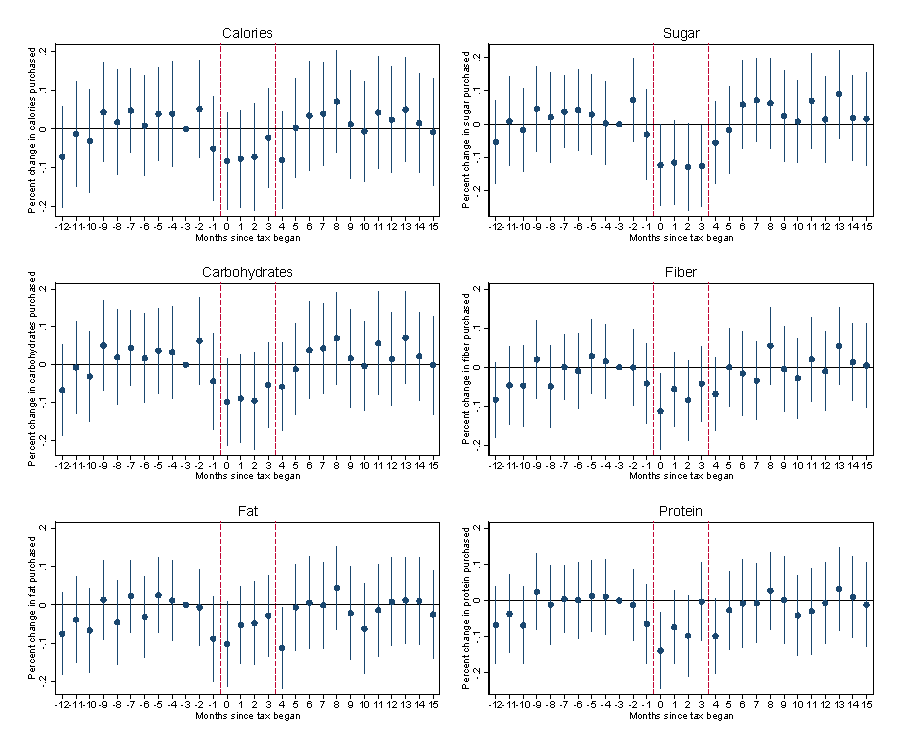
\includegraphics[width=1\textwidth, angle=0]{../figures/coefplot_cook_combo.pdf}
\footnotesize Each panel displays the monthly differences in log quantities purchased by residents of Cook County, Illinois and those in the same DMA outside of the county limits. The regressions used include household and month fixed-effects, and errors are clustered and the zip-code level. Vertical dashed lines represent the start and end of the tax in Cook County.
\end{center}
\end{figure}

\clearpage
\begin{figure}[t]\centering
\caption{Cook County zip code layers} \label{cookzip}
	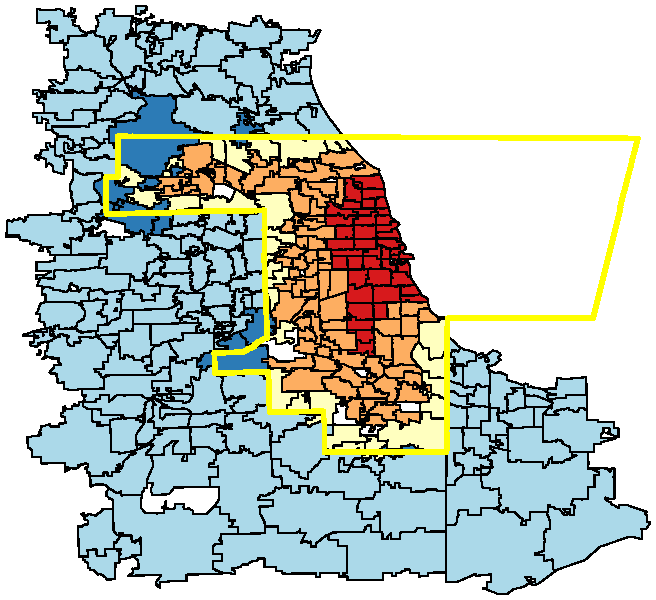
\includegraphics[width = \textwidth]{../figures/cookzips.pdf}
	\footnotesize Zip code layers used for examining heterogeneous treatment effects by distance from the nearest border. White regions in the map have no corresponding zip code information (lakes, forest, and other land without mailing addresses) and hence are excluded from the analysis. The darkest blue zip codes contain households both inside and outside Cook County's border. The lighter-yellow zips lie on the border entirely within Cook County. The remaining layers are constructed using linear distance to the nearest untaxed zip.
\end{figure}

% Soda budget share
\clearpage
\begin{figure}[t]\centering
\caption{Soda budget share and price} \label{soda_price}
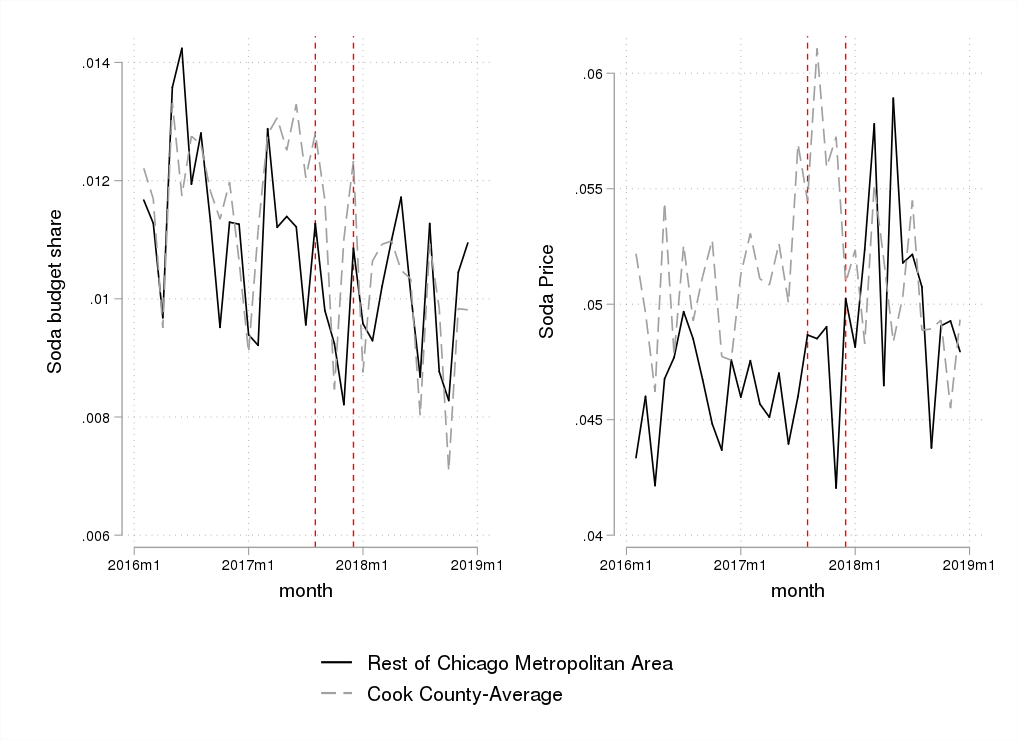
\includegraphics[width = \textwidth]{../figures/server_output/soda_price_and_share.png}
% \caption*{Source: Nielsen Consumer Panel}
\end{figure}

% Price indices
\clearpage
\begin{figure}[t]\centering
\caption{Price indices} \label{priceindex}
	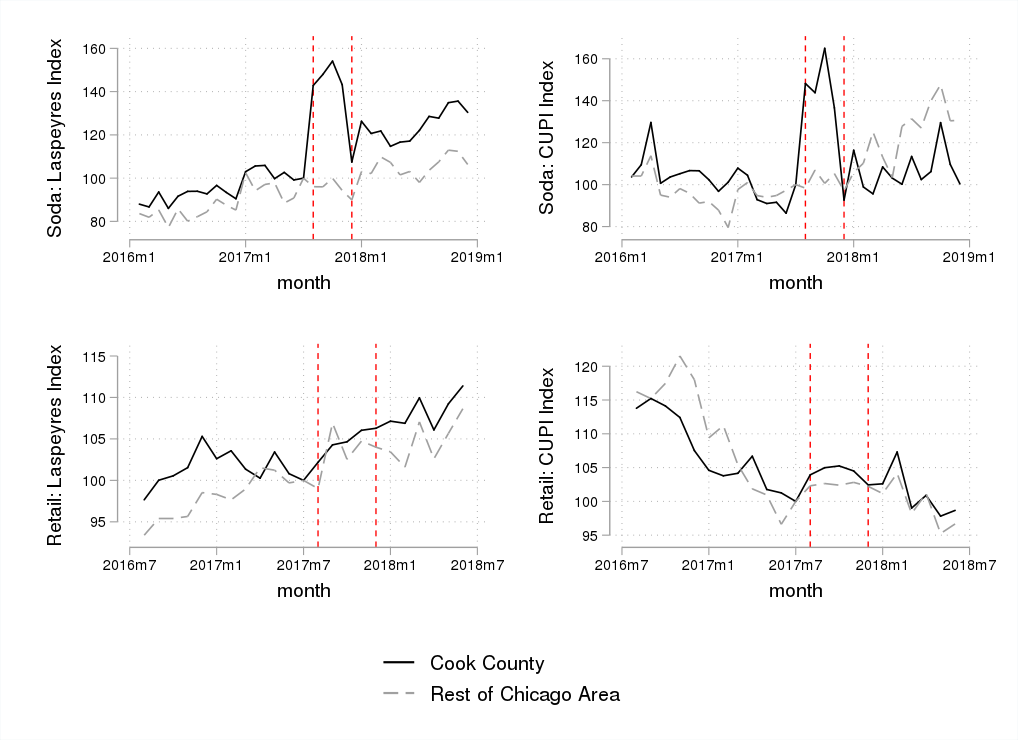
\includegraphics[width = \textwidth]{../figures/server_output/price_index_all.png}
	\caption*{Note: The top row shows the change in the soda only price index in Cook County and the rest of the Chicago Area. The bottom row shows the full retail price index. The right side assumes that households have nested CES preferences with time varying taste parameters, while the left hand-side is a simple Laspeyres weighted index. All price indices are set at 100 in July 2017. }
\end{figure}

% *****************************************************************
% Appendix
% *****************************************************************
\clearpage
\section*{Appendix}

\renewcommand{\thesubsection}{\Alph{subsection}}
\setcounter{table}{0}
\renewcommand{\thetable}{A\arabic{table}}
\setcounter{figure}{0}
\renewcommand{\thefigure}{A\arabic{figure}}

%%% TABLES

\begin{spacing}{1.0} 
\begin{table}[h] 
\centering
\caption{Summary statistics by soda decile, Cook County}
\label{summary_deciles} 
\begin{threeparttable}
\begin{tabular}{l*{1}{ccccccc}}
\toprule
                        &Reg. soda &   Sugar &Sugar from&       Trips&Items&Total spent&Hh.\\
            & (oz) & (g) & soda (g) & & scanned& (\$) & size\\
\midrule


\customlinespace Deciles 1 - 2       &        0.00&      442.04&        0.00&       11.45&       81.75&      456.29&        2.00\\
          &        (0.00)&      (448.05)&        (0.00)&        (9.51)&       (53.41)&      (362.63)&        (1.18)\\



\customlinespace Decile 3        &        7.38&      560.01&       11.62&       11.54&       99.98&      505.12&        2.12\\
          &       (23.59)&      (576.91)&       (48.87)&        (6.93)&       (62.91)&      (325.10)&        (1.15)\\



\customlinespace Decile 4        &       25.07&      674.40&       46.28&       14.25&      108.58&      567.62&        2.04\\
          &       (62.62)&      (603.01)&      (144.72)&        (9.97)&       (70.41)&      (392.79)&        (1.02)\\



\customlinespace Decile 5        &       52.11&      793.11&      110.68&       13.79&      117.54&      601.94&        2.31\\
          &      (120.54)&      (779.81)&      (350.65)&        (8.88)&       (75.19)&      (584.85)&        (1.30)\\



\customlinespace Decile 6        &       85.38&      861.31&      186.44&       15.49&      108.42&      584.54&        2.21\\
          &      (159.70)&      (902.21)&      (430.67)&       (14.58)&       (72.25)&      (426.79)&        (1.21)\\



\customlinespace Decile 7        &      133.10&      983.27&      293.43&       12.36&      114.14&      556.78&        2.64\\
          &      (215.90)&      (991.17)&      (628.80)&        (8.46)&       (74.32)&      (420.58)&        (1.34)\\



\customlinespace Decile 8        &      224.79&     1300.58&      575.75&       13.83&      116.80&      564.61&        2.39\\
          &      (290.68)&     (1274.11)&      (923.06)&        (9.86)&       (75.06)&      (401.53)&        (1.23)\\



\customlinespace Decile 9        &      371.25&     1743.45&      904.20&       14.15&      134.41&      558.40&        2.55\\
          &      (446.85)&     (1622.65)&     (1287.80)&       (11.24)&       (99.54)&      (421.21)&        (1.37)\\


\customlinespace Decile 10        &      729.56&     2490.04&     1959.81&       12.17&      114.15&      454.44&        2.28\\
          &      (704.40)&     (2035.11)&     (2259.00)&        (8.53)&       (73.93)&      (339.24)&        (1.26)\\

\bottomrule
\end{tabular}
\Fignote{Deciles are calculated using each household's average monthly
        soda volume purchased per dollar spent during the year prior to the tax,
        omitting the month prior to the tax. Standard deviations in parentheses.}
        \end{threeparttable} 
\end{table} 
\end{spacing}

\clearpage
\begin{spacing}{1.0} \begin{table} \centering \caption{Effects of tax on sugar by pretreatment soda quintile, Philadelphia} \label{sodatilesgphilly} \begin{threeparttable} \begin{tabular}{m{0.23\linewidth}*{6}{>{\centering\arraybackslash}m{0.10\linewidth}}} \toprule
                    & \multicolumn{3}{c}{DV: 4 months sugar} & \multicolumn{3}{c}{DV: 12 months sugar}\\
\cmidrule(l{.75em}){2-4} \cmidrule(l{.75em}){5-7} 
Pre-tax soda quintile&\multicolumn{1}{c}{(1)}         &\multicolumn{1}{c}{(2)}         &\multicolumn{1}{c}{(3)}         &\multicolumn{1}{c}{(4)}         &\multicolumn{1}{c}{(5)}         &\multicolumn{1}{c}{(6)}         \\
\midrule
\customlinespace Quintile 1 &       0.104         &       0.047         &       0.116         &       0.176         &       0.082         &       0.226\sym{*}  \\
                    &     (0.076)         &     (0.093)         &     (0.091)         &     (0.089)         &     (0.120)         &     (0.093)         \\
\customlinespace Quintile 2 &       0.225         &       0.328\sym{**} &       0.313\sym{*}  &       0.234\sym{*}  &       0.310\sym{**} &       0.378\sym{***}\\
                    &     (0.123)         &     (0.125)         &     (0.131)         &     (0.091)         &     (0.093)         &     (0.102)         \\
\customlinespace Quintile 3 &       0.077         &       0.032         &      -0.017         &       0.048         &       0.017         &      -0.011         \\
                    &     (0.078)         &     (0.097)         &     (0.102)         &     (0.077)         &     (0.091)         &     (0.103)         \\
\customlinespace Quintile 4 &      -0.251\sym{*}  &      -0.273         &      -0.236         &      -0.312\sym{***}&      -0.291\sym{***}&      -0.196\sym{*}  \\
                    &     (0.117)         &     (0.148)         &     (0.140)         &     (0.065)         &     (0.057)         &     (0.081)         \\
\customlinespace Quintile 5 &      -0.253         &      -0.278         &      -0.260         &      -0.252\sym{**} &      -0.252\sym{*}  &      -0.113         \\
                    &     (0.137)         &     (0.146)         &     (0.151)         &     (0.093)         &     (0.103)         &     (0.171)         \\
\midrule
Treated Households           &         262         &         262         &         148         &         284         &         284         &         122         \\
Households          &        2012         &        2012         &        1221         &        2214         &        2214         &        1000         \\
Household-months    &       26983         &       26983         &       19536         &       41776         &       41776         &       25000         \\
Household FEs             &         Yes         &         Yes         &         Yes         &         Yes         &         Yes         &         Yes         \\
Month FEs              &         Yes         &         Yes         &         Yes         &         Yes         &         Yes         &         Yes         \\
Balanced Panel             &          No         &          No         &         Yes         &          No         &          No         &         Yes         \\
Sampling Weights             &          No         &         Yes         &         Yes         &          No         &         Yes         &         Yes         \\
\bottomrule \end{tabular} \Fignote{Coefficients represent the percent change in sugar purchased during the first four months (1 - 3) and year (4 - 6) after the Philadelphia beverage tax became active, separated by pretreatment regular soda volume purchase decile. Quintiles were calculated based on the treated households' average monthly volume of soda purchased during the previous year omitting the month prior to the tax. Nearly all of quintile 1 report zero regular soda purchases before the tax. \Regnote} \end{threeparttable} \end{table} \end{spacing}


\clearpage
\begin{spacing}{1.0} \begin{table} \centering \caption{Effects of tax on sugar by pretreatment soda quintile, Seattle and San Francisco} \label{sodatilesgsf} \begin{threeparttable} \begin{tabular}{m{0.23\linewidth}*{6}{>{\centering\arraybackslash}m{0.10\linewidth}}} \toprule
                    & \multicolumn{3}{c}{Months 1 - 4, sugar} & \multicolumn{3}{c}{Months 5 - 8, sugar}\\
\cmidrule(l{.75em}){2-4} \cmidrule(l{.75em}){5-7} 
Pre-tax soda quintile&\multicolumn{1}{c}{(1)}         &\multicolumn{1}{c}{(2)}         &\multicolumn{1}{c}{(3)}         &\multicolumn{1}{c}{(4)}         &\multicolumn{1}{c}{(5)}         &\multicolumn{1}{c}{(6)}         \\
\midrule
\customlinespace Quintiles 1 - 2 &       0.053         &      -0.144         &      -0.172         &       0.065         &      -0.001         &       0.093         \\
                    &     (0.085)         &     (0.142)         &     (0.142)         &     (0.097)         &     (0.135)         &     (0.138)         \\
\customlinespace Quintile 3 &       0.150         &       0.099         &       0.070         &       0.061         &       0.258         &       0.187         \\
                    &     (0.129)         &     (0.148)         &     (0.164)         &     (0.144)         &     (0.193)         &     (0.211)         \\
\customlinespace Quintile 4 &      -0.021         &      -0.116         &      -0.172         &      -0.180         &      -0.336         &      -0.337         \\
                    &     (0.105)         &     (0.139)         &     (0.148)         &     (0.156)         &     (0.218)         &     (0.238)         \\
\customlinespace Quintile 5 &      -0.473\sym{**} &      -0.596\sym{**} &      -0.613\sym{**} &      -0.098         &      -0.128         &      -0.161         \\
                    &     (0.148)         &     (0.229)         &     (0.237)         &     (0.102)         &     (0.189)         &     (0.201)         \\
\midrule
Treated Households           &         229         &         229         &         153         &         229         &         229         &         151         \\
Households          &        2141         &        2141         &        1402         &        2141         &        2141         &        1375         \\
Household-months    &       27663         &       27663         &       21030         &       34932         &       34932         &       26125         \\
Balanced Panel             &          No         &          No         &         Yes         &          No         &          No         &         Yes         \\
Sampling Weights             &          No         &         Yes         &         Yes         &          No         &         Yes         &         Yes         \\
\bottomrule \end{tabular} \Fignote{Coefficients represent the percent change in sugar purchased during the first four months (1 - 3) and second four months (4 - 6) after the Seattle and San Francisco beverage taxes became active, separated by expenditure-weighted pretreatment regular soda volume purchase decile. We omit the month prior to the tax to reduce bias from anticipatory effects. Quintiles were calculated based on the treated households' average monthly volume of soda purchased during the previous year omitting the month prior to the tax. All of quintile 1 and nearly all of quintile 2 report zero regular soda purchases before the tax. \Regnote} \end{threeparttable} \end{table} \end{spacing}


\clearpage
\begin{spacing}{1.0} \begin{table} \centering \caption{Effects of Cook County Beverage Tax on nutrients, 10 largest counties by population as counterfactual} \label{itt_cook_nutrients_counties_largest} \begin{threeparttable} \begin{tabular}{m{0.23\linewidth}*{6}{>{\centering\arraybackslash}m{0.10\linewidth}}} \toprule
            & \multicolumn{3}{c}{During tax} & \multicolumn{3}{c}{4 months post tax}\\
\cmidrule(l{.75em}){2-4} \cmidrule(l{.75em}){5-7} 
Dependent Variable&\multicolumn{1}{c}{(1)}         &\multicolumn{1}{c}{(2)}         &\multicolumn{1}{c}{(3)}         &\multicolumn{1}{c}{(4)}         &\multicolumn{1}{c}{(5)}         &\multicolumn{1}{c}{(6)}         \\
\midrule 
\customlinespace 

All sugar  &      -0.129\sym{***}&      -0.087\sym{*}  &      -0.095\sym{*}  &       0.020         &       0.056         &       0.072         \\
            &     (0.031)         &     (0.040)         &     (0.043)         &     (0.030)         &     (0.036)         &     (0.039)         \\
\customlinespace 

Carbohydrates  &      -0.069\sym{*}  &      -0.027         &      -0.031         &       0.020         &       0.048         &       0.052         \\
            &     (0.029)         &     (0.037)         &     (0.039)         &     (0.028)         &     (0.034)         &     (0.035)         \\
\customlinespace 

Carb., non-sugar&       0.033         &       0.061         &       0.056         &       0.042         &       0.062         &       0.053         \\
            &     (0.032)         &     (0.038)         &     (0.043)         &     (0.031)         &     (0.039)         &     (0.040)         \\
\customlinespace 

Calories    &      -0.035         &       0.003         &      -0.003         &       0.018         &       0.044         &       0.043         \\
            &     (0.031)         &     (0.039)         &     (0.041)         &     (0.029)         &     (0.036)         &     (0.035)         \\
\customlinespace 

Calories, non-sugar&       0.028         &       0.056         &       0.059         &       0.028         &       0.042         &       0.047         \\
            &     (0.037)         &     (0.046)         &     (0.045)         &     (0.033)         &     (0.047)         &     (0.041)         \\
\customlinespace 

Fat    &       0.007         &       0.053         &       0.052         &       0.027         &       0.052         &       0.044         \\
            &     (0.026)         &     (0.033)         &     (0.033)         &     (0.024)         &     (0.034)         &     (0.034)         \\
\customlinespace 

Fiber  &      -0.011         &       0.037         &       0.034         &       0.041         &       0.069\sym{*}  &       0.062\sym{*}  \\
            &     (0.023)         &     (0.028)         &     (0.030)         &     (0.024)         &     (0.030)         &     (0.031)         \\
\customlinespace 

Protein&      -0.010         &       0.030         &       0.031         &       0.030         &       0.059         &       0.061         \\
            &     (0.027)         &     (0.032)         &     (0.034)         &     (0.026)         &     (0.035)         &     (0.034)         \\
\customlinespace 

Sodium &      -0.031         &       0.000         &       0.013         &       0.040\sym{*}  &       0.053\sym{*}  &       0.055\sym{*}  \\
            &     (0.021)         &     (0.024)         &     (0.025)         &     (0.020)         &     (0.025)         &     (0.026)         \\
\customlinespace 

\midrule 
Treated Households   &        1142         &        1142         &         719         &        1220         &        1220         &         624         \\
Households  &        7464         &        7464         &        4453         &        8250         &        8250         &        3804         \\
Household-months&       92291         &       92291         &       66795         &       91334         &       91334         &       57060         \\
Balanced Panel     &          No         &          No         &         Yes         &          No         &          No         &         Yes         \\
Sampling Weights     &          No         &         Yes         &         Yes         &          No         &         Yes         &         Yes         \\
\bottomrule \end{tabular} \Fignote{Coefficients represent the percent change in the dependent variable during the four months that the Cook County beverage tax was active (1 - 3) and the four months after the tax was no longer active (4 - 6) relative to the 12 months preceding the tax, omitting the month prior to the tax. \FEnote \Regnote} \end{threeparttable} \end{table} \end{spacing}


\clearpage
\begin{spacing}{1.0} \begin{table} \centering \caption{Effects of Cook County Beverage Tax on nutrients, 10 nearest population density counties as counterfactual} \label{itt_cook_nutrients_counties_dense} \begin{threeparttable} \begin{tabular}{m{0.23\linewidth}*{6}{>{\centering\arraybackslash}m{0.10\linewidth}}} \toprule
            & \multicolumn{3}{c}{During tax} & \multicolumn{3}{c}{4 months post tax}\\
\cmidrule(l{.75em}){2-4} \cmidrule(l{.75em}){5-7} 
Dependent Variable&\multicolumn{1}{c}{(1)}         &\multicolumn{1}{c}{(2)}         &\multicolumn{1}{c}{(3)}         &\multicolumn{1}{c}{(4)}         &\multicolumn{1}{c}{(5)}         &\multicolumn{1}{c}{(6)}         \\
\midrule 
\customlinespace 

All sugar  &      -0.117\sym{**} &      -0.138\sym{**} &      -0.104\sym{*}  &      -0.016         &       0.029         &       0.083         \\
            &     (0.039)         &     (0.050)         &     (0.052)         &     (0.039)         &     (0.050)         &     (0.058)         \\
\customlinespace 

Carbohydrates  &      -0.089\sym{*}  &      -0.113\sym{*}  &      -0.072         &      -0.032         &       0.004         &       0.047         \\
            &     (0.037)         &     (0.047)         &     (0.048)         &     (0.037)         &     (0.048)         &     (0.056)         \\
\customlinespace 

Carb., non-sugar&      -0.022         &      -0.047         &      -0.008         &      -0.038         &      -0.002         &       0.013         \\
            &     (0.049)         &     (0.054)         &     (0.057)         &     (0.050)         &     (0.056)         &     (0.065)         \\
\customlinespace 

Calories    &      -0.062         &      -0.085         &      -0.046         &      -0.045         &      -0.002         &       0.037         \\
            &     (0.038)         &     (0.048)         &     (0.049)         &     (0.039)         &     (0.051)         &     (0.057)         \\
\customlinespace 

Calories, non-sugar&      -0.001         &      -0.033         &       0.028         &      -0.029         &       0.030         &       0.053         \\
            &     (0.051)         &     (0.056)         &     (0.056)         &     (0.049)         &     (0.066)         &     (0.066)         \\
\customlinespace 

Fat    &       0.005         &       0.002         &       0.044         &      -0.028         &       0.016         &       0.048         \\
            &     (0.033)         &     (0.043)         &     (0.045)         &     (0.034)         &     (0.046)         &     (0.053)         \\
\customlinespace 

Fiber  &      -0.014         &      -0.021         &      -0.003         &      -0.024         &       0.007         &       0.032         \\
            &     (0.033)         &     (0.040)         &     (0.043)         &     (0.033)         &     (0.043)         &     (0.048)         \\
\customlinespace 

Protein&      -0.029         &      -0.034         &       0.005         &      -0.033         &       0.023         &       0.065         \\
            &     (0.035)         &     (0.042)         &     (0.044)         &     (0.038)         &     (0.051)         &     (0.058)         \\
\customlinespace 

Sodium &      -0.013         &      -0.010         &       0.025         &      -0.003         &       0.027         &       0.059         \\
            &     (0.026)         &     (0.032)         &     (0.034)         &     (0.027)         &     (0.036)         &     (0.043)         \\
\customlinespace 

\midrule 
Treated Households   &        1142         &        1142         &         719         &        1220         &        1220         &         624         \\
Households  &        1907         &        1907         &        1202         &        2059         &        2059         &        1029         \\
Household-months&       24004         &       24004         &       18030         &       23630         &       23630         &       15435         \\
Balanced Panel     &          No         &          No         &         Yes         &          No         &          No         &         Yes         \\
Sampling Weights     &          No         &         Yes         &         Yes         &          No         &         Yes         &         Yes         \\
\bottomrule \end{tabular} \Fignote{Coefficients represent the percent change in the dependent variable during the four months that the Cook County beverage tax was active (1 - 3) and the four months after the tax was no longer active (4 - 6) relative to the 12 months preceding the tax, omitting the month prior to the tax. \FEnote \Regnote} \end{threeparttable} \end{table} \end{spacing}


%%% FIGURES

% Cook Co: Panelist nutrition
\clearpage
\begin{figure}[t]
\begin{center}
\caption{Cook County DMA: nutrient composition over time}
\label{cook_panelist_nutr}
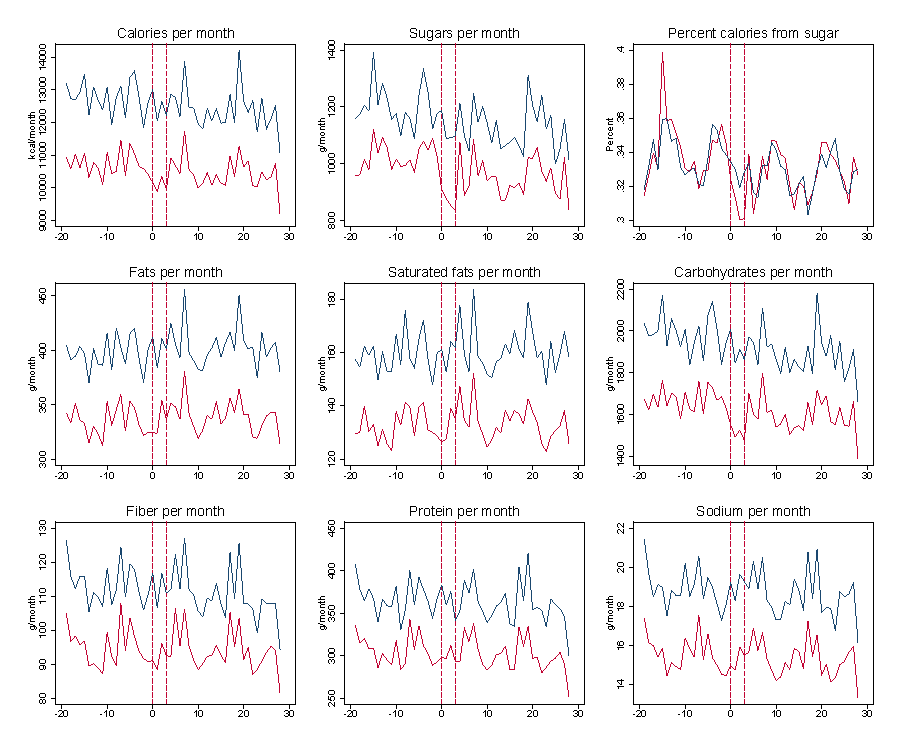
\includegraphics[width=1\textwidth, angle=0]{../figures/panelist_nutr.pdf}
\footnotesize Each panel displays monthly sums or percentages of different nutrients for residents of Cook County, Illinois (red) and those in the same DMA outside of the county limits (blue). Vertical dashed lines represent the start and end of the tax in Cook County.
\end{center}
\end{figure}

% Cook Co: Panelist behaviors
\clearpage
\begin{figure}[t]
\begin{center}
\caption{Cook County DMA: panelist behaviors over time}
\label{cook_panelist_behav}
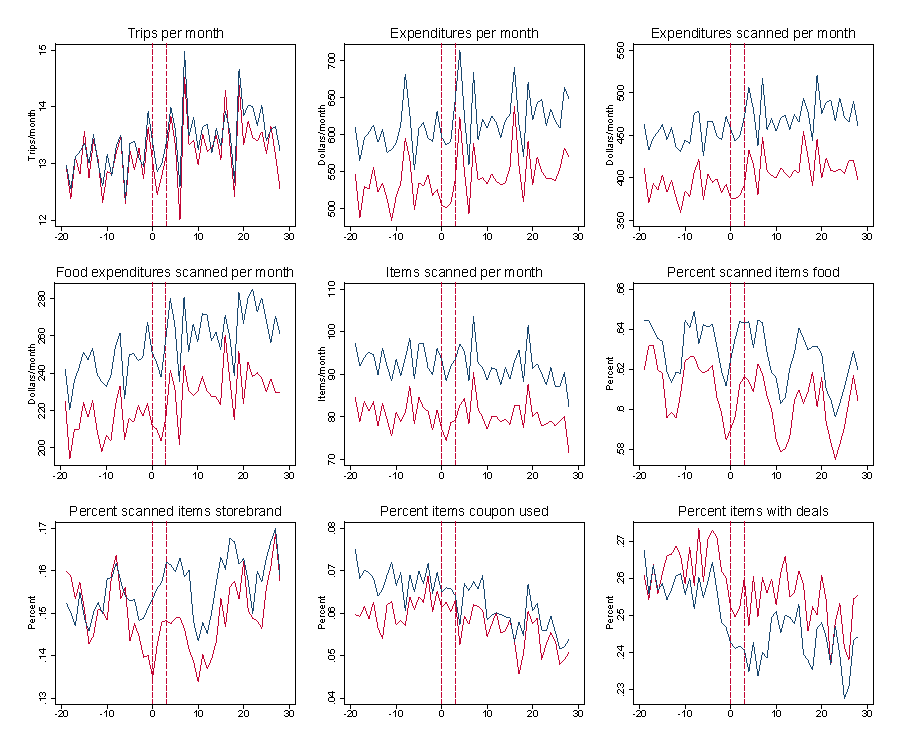
\includegraphics[width=1\textwidth, angle=0]{../figures/panelist_behav.pdf}
\footnotesize Each panel displays monthly sums or percentages of panelist behaviors for residents of Cook County, Illinois (red) and those in the same DMA outside of the county limits (blue). Vertical dashed lines represent the start and end of the tax in Cook County.
\end{center}
\end{figure}

% Cook Co: Panelist beverages
\clearpage
\begin{figure}[t]
\begin{center}
\caption{Cook County DMA: beverage purchases over time}
\label{cook_panelist_bev}
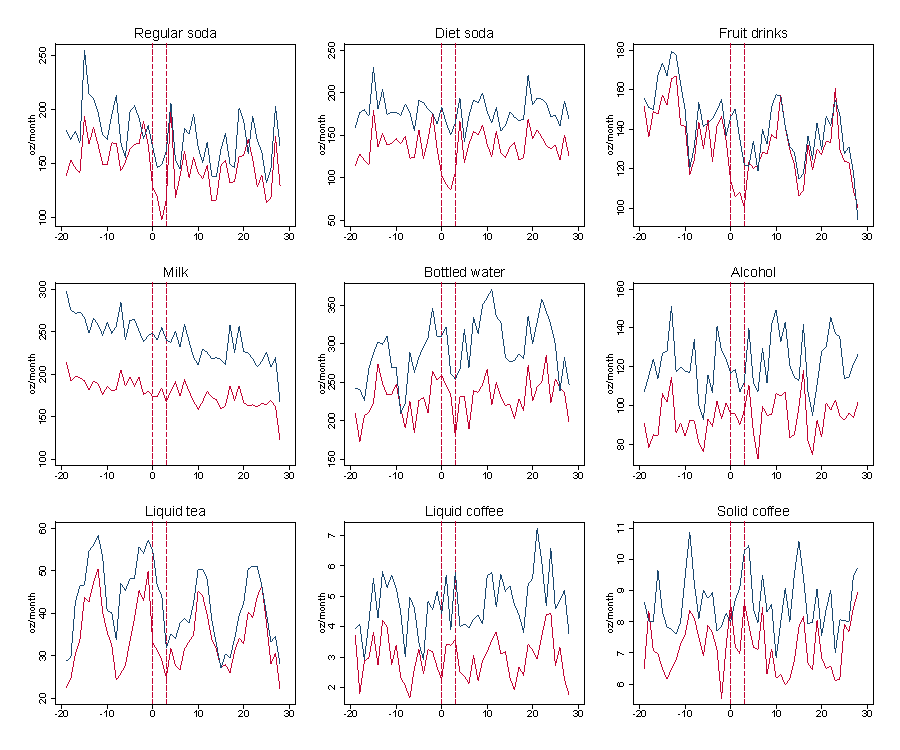
\includegraphics[width=1\textwidth, angle=0]{../figures/panelist_bev.pdf}
\footnotesize Each panel displays monthly sums of purchased beverages (in ounces) for residents of Cook County, Illinois (red) and those in the same DMA outside of the county limits (blue). Vertical dashed lines represent the start and end of the tax in Cook County.
\end{center}
\end{figure}

% Cook Co: Panelist sugar by source
\clearpage
\begin{figure}[t]
\begin{center}
\caption{Cook County DMA: sugar by source over time}
\label{cook_panelist_sugar_sources}
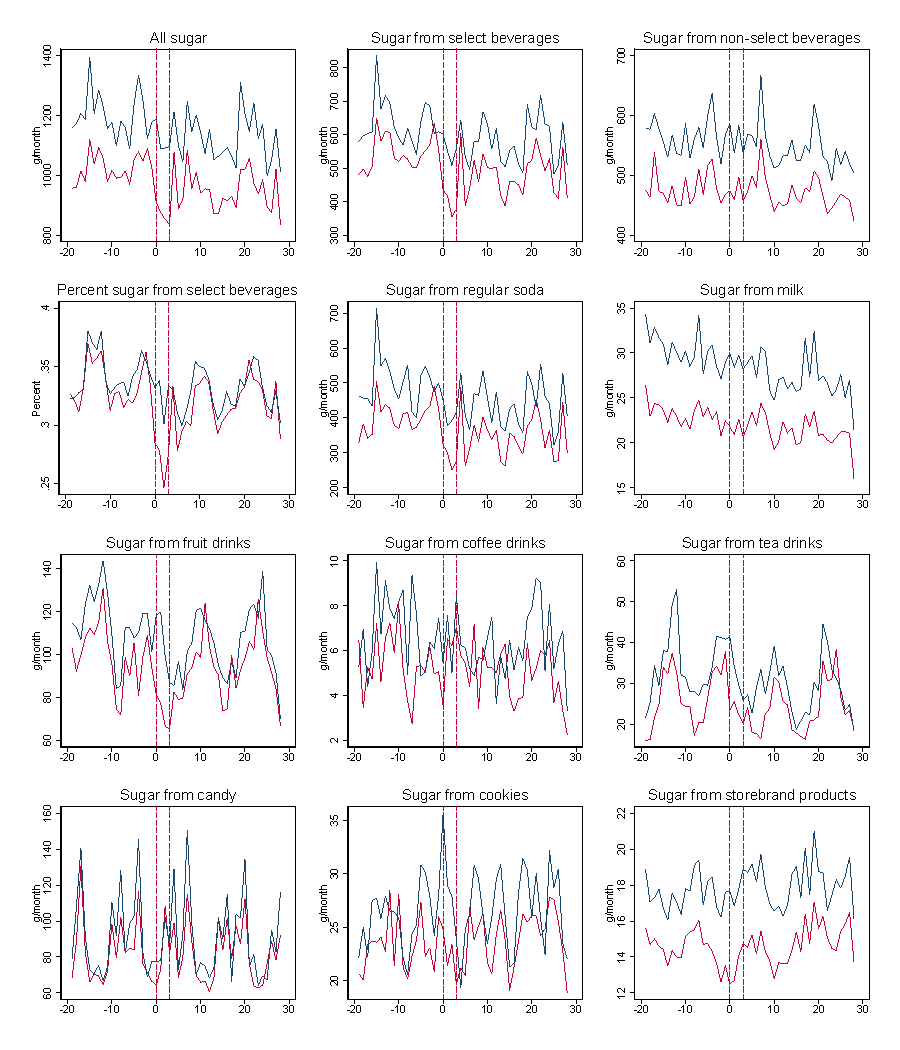
\includegraphics[width=1\textwidth, angle=0]{../figures/panelist_sugar_sources.pdf}
\footnotesize Each panel displays monthly sums of sugar (in grams) for residents of Cook County, Illinois (red) and those in the same DMA outside of the county limits (blue) from different product groups. Vertical dashed lines represent the start and end of the tax in Cook County.
\end{center}
\end{figure}

% Cook Co: Panelist sugar by store location
\clearpage
\begin{figure}[t]
\begin{center}
\caption{Cook County DMA: variation by store location}
\label{cook_panelist_stores}
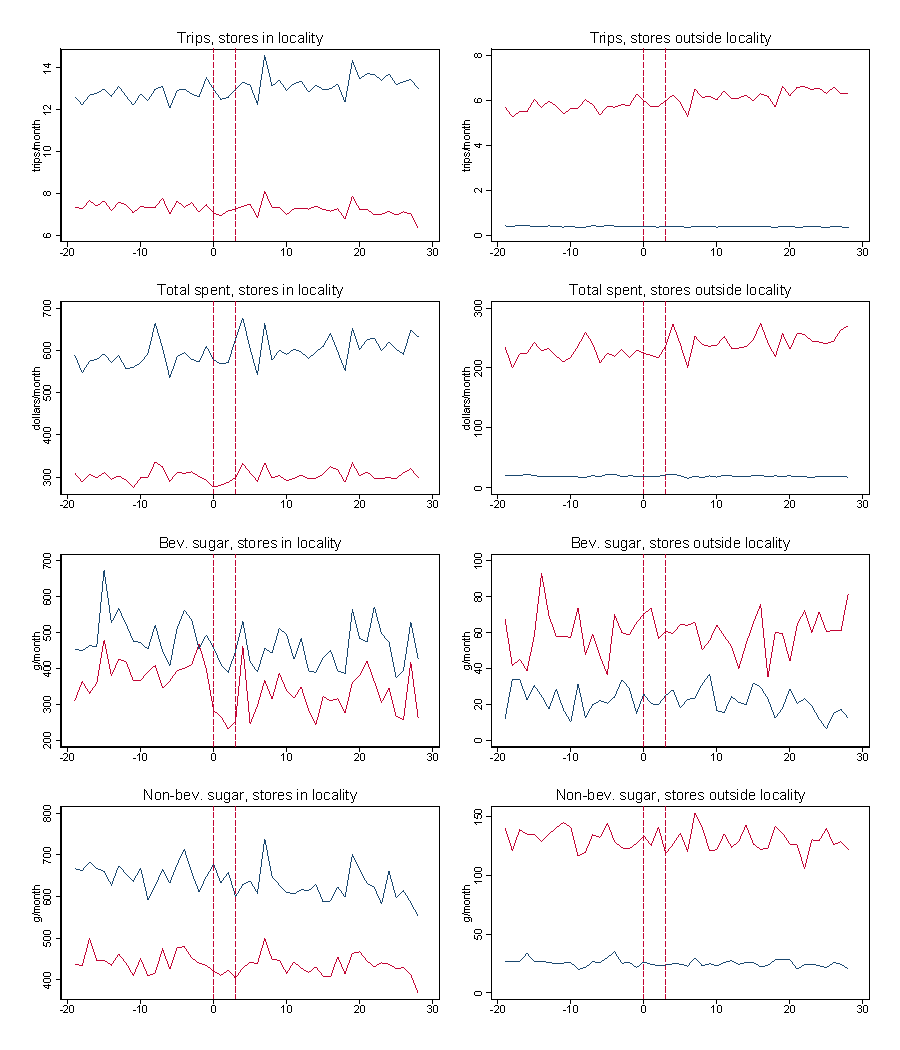
\includegraphics[width=0.95\textwidth, angle=0]{../figures/panelist_cook_stores.pdf}
\footnotesize Each panel displays monthly sums of trips, total purchases, and grams of sugar (from beverages or non-beverages) for residents of Cook County, Illinois (red) and those in the same DMA outside of the county limits (blue). Left panels are sums within Cook County stores for Cook County residents and non-Cook County stores for control residents. Right panels show the reverse: sums within non-Cook County stores for Cook County residents and Cook County stores for control residents. Vertical dashed lines represent the start and end of the tax in Cook County.
\end{center}
\end{figure}

% Cook Co: Panelist nutrition, large county counterfactual
\clearpage
\begin{figure}[t]
\begin{center}
\caption{Cook County DMA: nutrient composition over time, ten largest counties as counterfactual}
\label{cook_panelist_nutr_counties_largest}
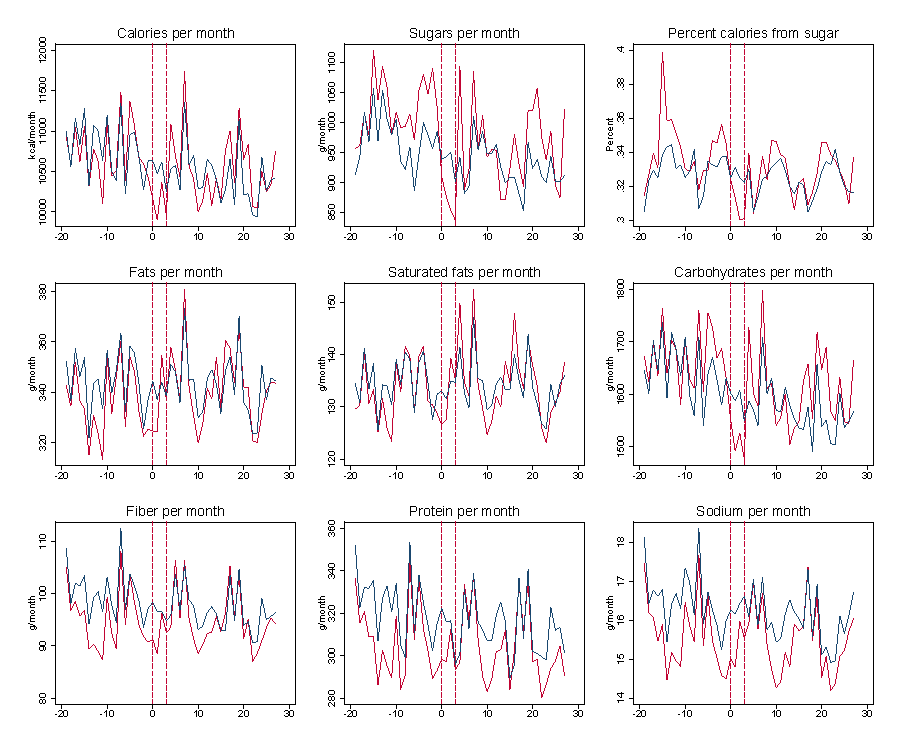
\includegraphics[width=1\textwidth, angle=0]{../figures/panelist_nutr_counties_largest.pdf}
\footnotesize Each panel displays monthly sums or percentages of different nutrients for residents of Cook County, Illinois (red) and those in the ten largest counties by population, excluding Cook County (blue). Vertical dashed lines represent the start and end of the tax in Cook County.
\end{center}
\end{figure}

% Cook Co: Panelist nutrition, dense county counterfactual
\clearpage
\begin{figure}[t]
\begin{center}
\caption{Cook County DMA: nutrient composition over time, ten nearest population density counties as counterfactual}
\label{cook_panelist_nutr_counties_dense}
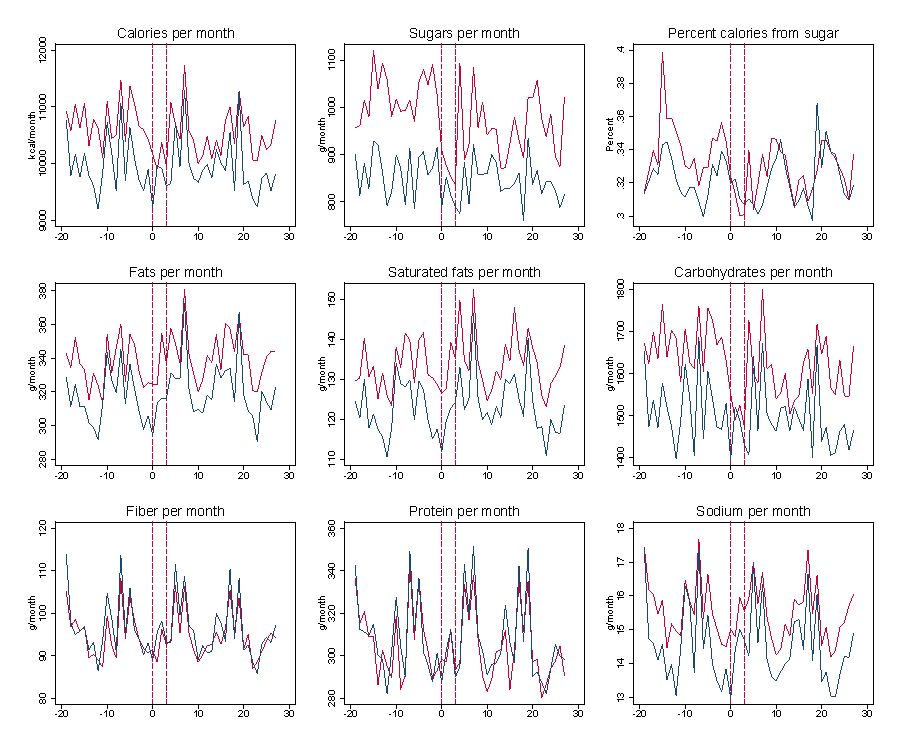
\includegraphics[width=1\textwidth, angle=0]{../figures/panelist_nutr_counties_dense.pdf}
\footnotesize Each panel displays monthly sums or percentages of different nutrients for residents of Cook County, Illinois (red) and those in the ten nearest counties by population density to Cook County (blue). Vertical dashed lines represent the start and end of the tax in Cook County.
\end{center}
\end{figure}

\begin{figure}[t]\centering
\caption{Example price tag from Cook County grocery store} \label{pricetag}
	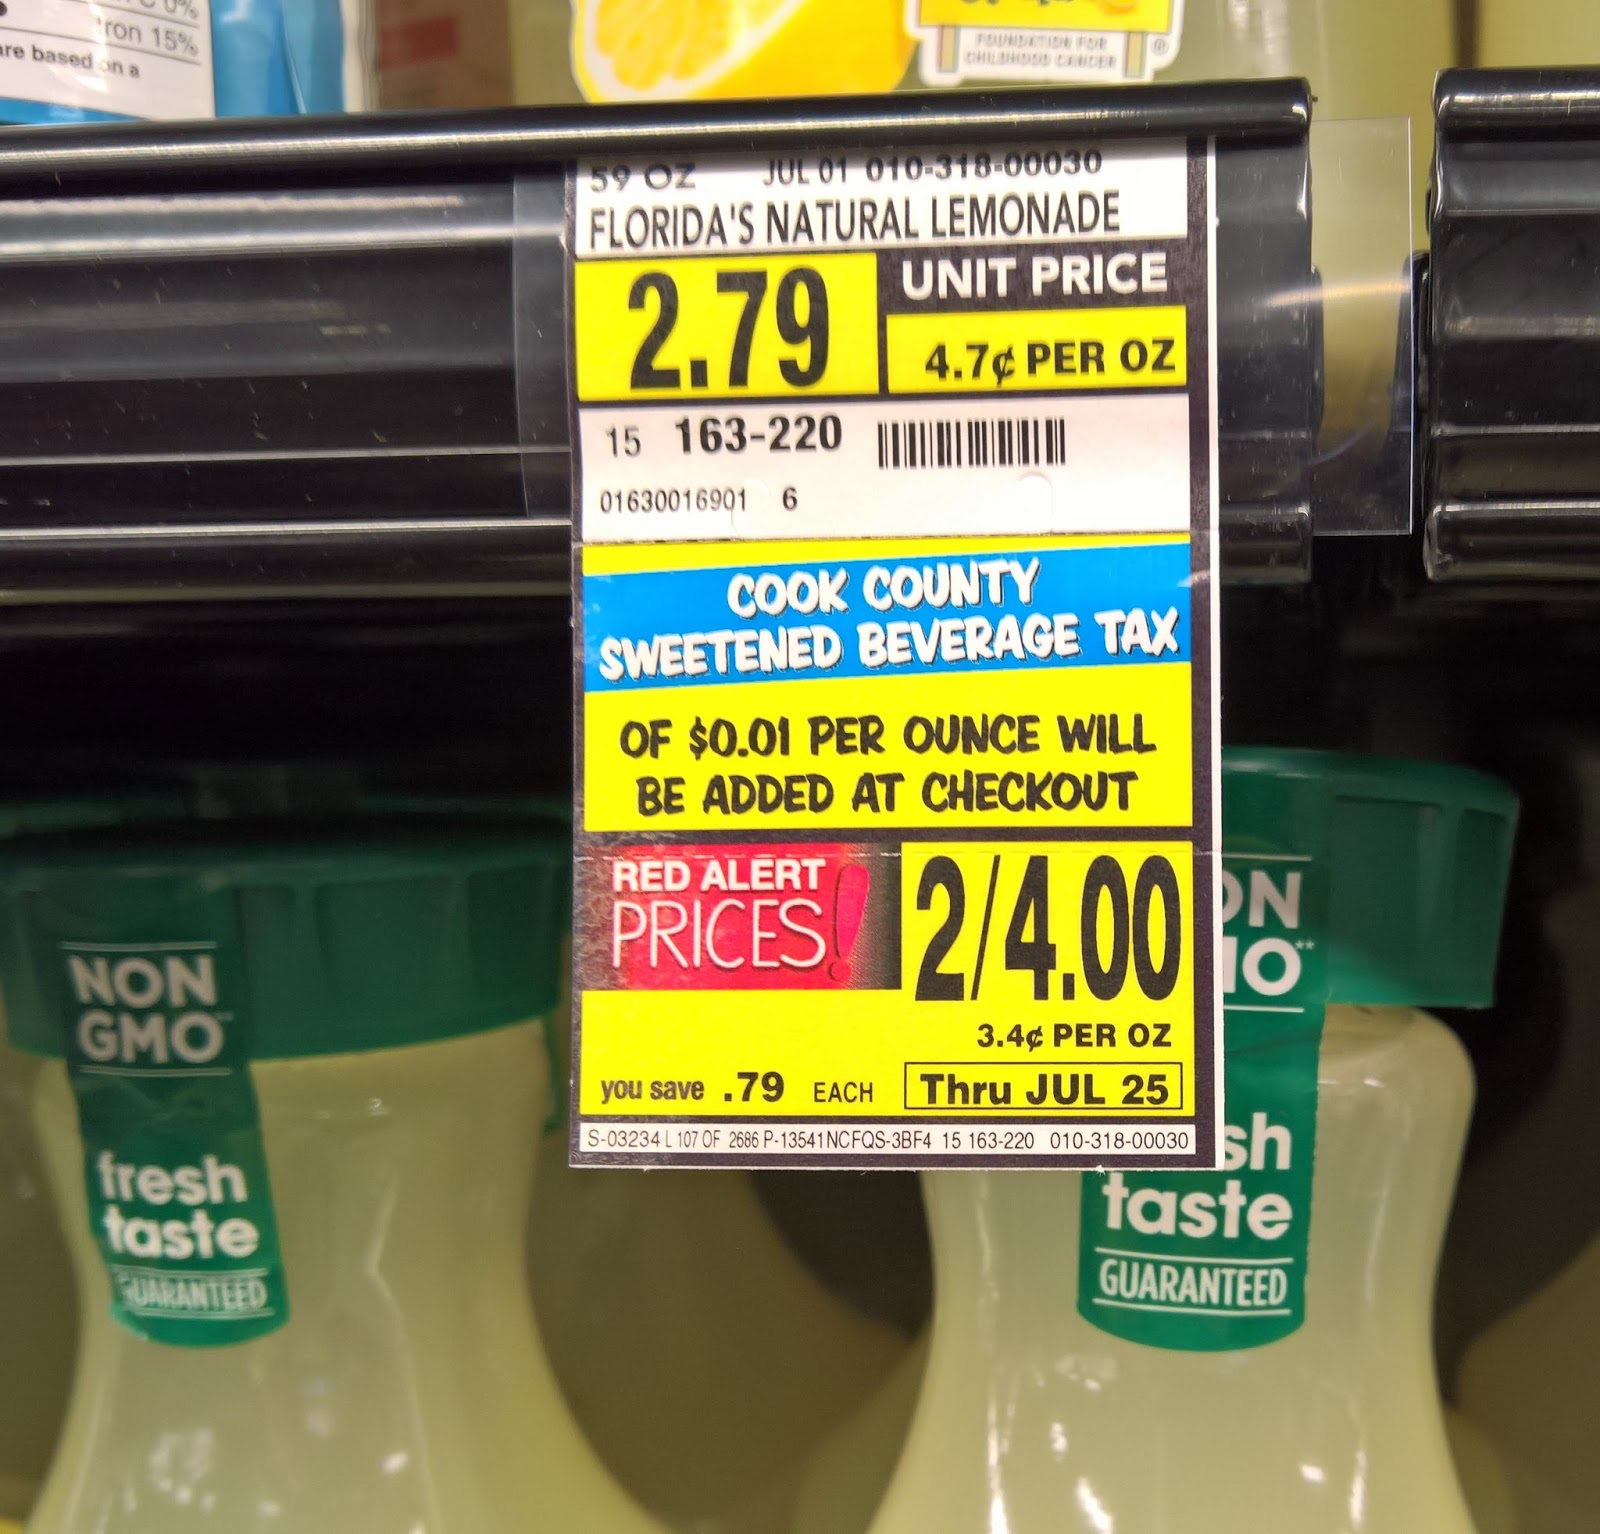
\includegraphics[width = \textwidth]{../figures/pricetag.jpg}
	\footnotesize This price tag includes a warning about the beverage tax in Cook County. Price tags like these may have increased salience of the tax whereas price tags in smaller, non-chain stores may not have.
\end{figure}

\clearpage
\begin{figure}[t]\centering
	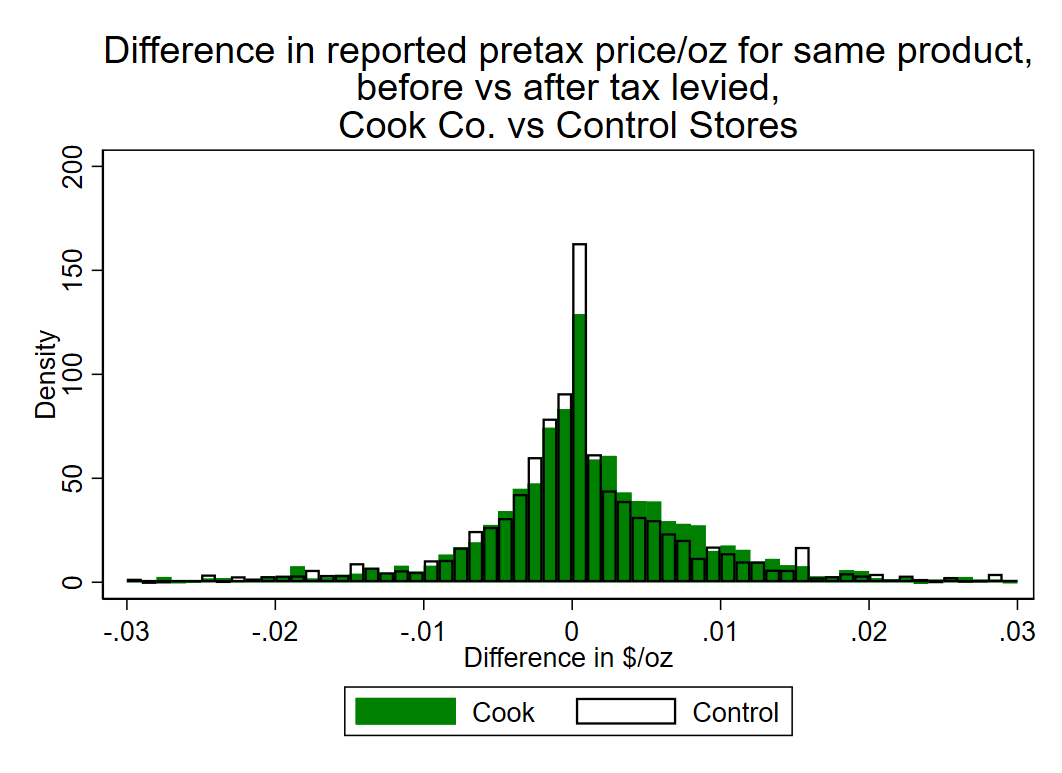
\includegraphics[width = \textwidth]{../figures/ppozdiff.png}\label{pricediff}
	\caption{Distribution of differences in price per ounce during pretax versus taxed periods for carbonated beverages}
\end{figure}

\clearpage
\begin{figure}[t]\centering
\caption{Relative weekly search volume for ``soda tax"}
\label{gtrends}
	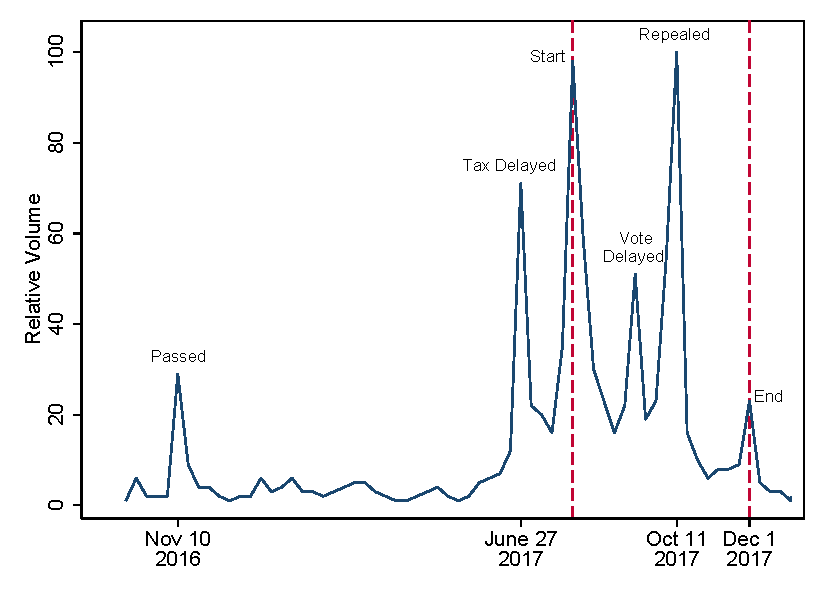
\includegraphics[width = \textwidth]{../figures/gtrends.pdf}
	\footnotesize This plot displays Google search volume in Illinois for the keywords ``soda tax". Each point is the volume in Illinois relative to the total search volume for that week in Illinois scaled so that the highest week's search volume is 100.
\end{figure}

\end{document}
